\RequirePackage{lineno}
\documentclass[aps,prl,reprint,twocolumn,groupedaddress,showpacs]{revtex4-1}
%\documentclass[aps,prl,reprint,twocolumn,groupedaddress,showpacs]{revtex4}
%\documentclass[10pt,reprint]{iopart}
%\documentclass[11pt]{article}
%\documentclass{pnastwo}
%\usepackage{color}
\usepackage[pdftex,draft]{graphicx}
\usepackage{epstopdf}
\usepackage{bm}
\usepackage{amssymb}
\usepackage{psfrag}
\usepackage{color}
\usepackage{amsbsy}      
\usepackage{amsmath,amsthm}
\usepackage{mathtools}
\usepackage{lineno}
\usepackage{natbib} 
\bibliographystyle{unsrt}
\graphicspath{{./figures/}}
%\usepackage{MnSymbol}

\newtheorem{thm}{Theorem}%
\newtheorem{lem}[thm]{Lemma}%
\newtheorem{prop}[thm]{Proposition}%
\newtheorem{coro}[thm]{Corollary}%
\DeclarePairedDelimiter{\norm}{\lVert}{\rVert}

\newcommand{\bsigma}{{\boldsymbol\sigma}}
\def\alphaeff{\alpha_{\mathrm{eff}}}
\def\a{\alpha}
\def\b{{\bf b}}
\def\c{{\bf c}}
\def\d{{\bf d}}
\def\dd{\mbox{d}}
\def\dz{\delta z}
\def\ve{\varepsilon}
\def\eps{\epsilon}
\def\f{{\bf f}}
\def\g{\gamma}
\def\r{{\bf r}}
\def\rp{{\bf r}_{\perp}}
\def\q{{\bf q}}
\def\k{\kappa}
\def\u{{\bf u}}
\def\t{{\bf t}}
\def\w{{\bf w}}
\def\x{{\bf x}}
\def\y{{\bf y}}
\def\l{\ell}
\def\o{\omega}
\def\p{{\bf p}}
\def\s{\sigma}
\def\vp{\varphi}
\def\D{\Delta}
\def\F{{\bf F}}
\def\H{{\bf H}}
\def\K{{\bf K}}
\def\L{{\bf L}}
\def\Q{{\bf Q}}
\def\S{{\bf S}}
\def\T{{\bf T}}
\def\U{{\bf U}}
\def\V{{\bf V}}
\def\W{{\bf W}}  
\def\F{{\bf F}}                
\def\P{{\bf P}}
\def\Pt{\tilde{P}}
%\def\s{\mathbf{\sigma}}
\newcommand{\bs}{\boldsymbol{\sigma}}
\newcommand{\Conv}{\mathop{\scalebox{1.5}{\raisebox{-0.2ex}{$\ast$}}}}%

%\usepackage{fullpage}
\newcommand{\RR}{\mathbb{R}}


\begin{document}

\title{Reconstruction of localized force distributions in cells and tissues from substrate displacements using physically-consistent regularization}

\author{Joshua C. Chang and Yanli Liu and Tom Chou} 
\affiliation{Epidemiology and Biostatistics Section, Rehabilitation Medicine, Clinical Center, The National Institutes of Health, Bethesda MD, 20892}
\affiliation{Depts. of
Biomathematics and Mathematics, UCLA, Los Angeles, CA 90095-1766}


%\maketitle 

%\begin{article}


%\runninglinenumbers*

\begin{abstract}
We develop a method to reconstruct, from measured displacements of the
underlying elastic substrate, the spatially dependent forces that
cells or tissues impart on it. Since these sources of force typically
arise from focal adhesions, with are localized and can exit only
within the footprint of the cell or tissue, they are compactly
supported. We solve this inverse problem using methods of $L^{1}$
optimization often used in image segmentation. In addition to the
standard quadratic data mismatch terms that defines least-squares
fitting, we motivate a term in the objective function which penalizes
variations in the tensor invariants of the reconstructed stress while
preserving boundaries.  By minimizing the objective function subject
to appropriate physical constraints, we are able to efficiently
reconstruct stress fields with localized structure from simulated and
experimental substrate displacements. We provide a numerical method
for setting up a discretized inverse problem that that is solvable by
standard convex optimization techniques. Our method incorporates the
exact solution of the forward problem accurate to first-order
finite-difference approximation in the stress tensor. Given
newly-available high-resolution data, we motivate the use of
distance-based cutoffs for data inclusion and find under loose
regularity conditions the reconstruction error that results.
\end{abstract}
\maketitle

\section{Introduction}

The adhesion of cells and tissues to their environment has profound
consequences on processes such as cell polarization \cite{MASHA},
motion, division, differentiation, tissue morphology during
development, and wound healing. Hence, quantifying how cells attach to
an impart force on the surrounding material is an important technical
challenge in cell biology.

Cell motility and response to signals have hitherto typically been
studied in two-dimensional geometries in which cells are placed on a
flat elastic substrate.  Dynamic adhesion between the cells and the
substrate are realized through {\it e.g.}, lamellapodia, filapodia,
and dynamically reorganizing focal adhesions.  Such structures are
spatially localized, as shown in Fig.~\ref{FIG1}. Similarly, on larger
length scales, a collection of cells can give rise to localized stress
distributions. For example, the leading edge of a cell layer produces
the pulling force that leads to migration in wound healing assays.

\begin{figure}[t]
\begin{center}
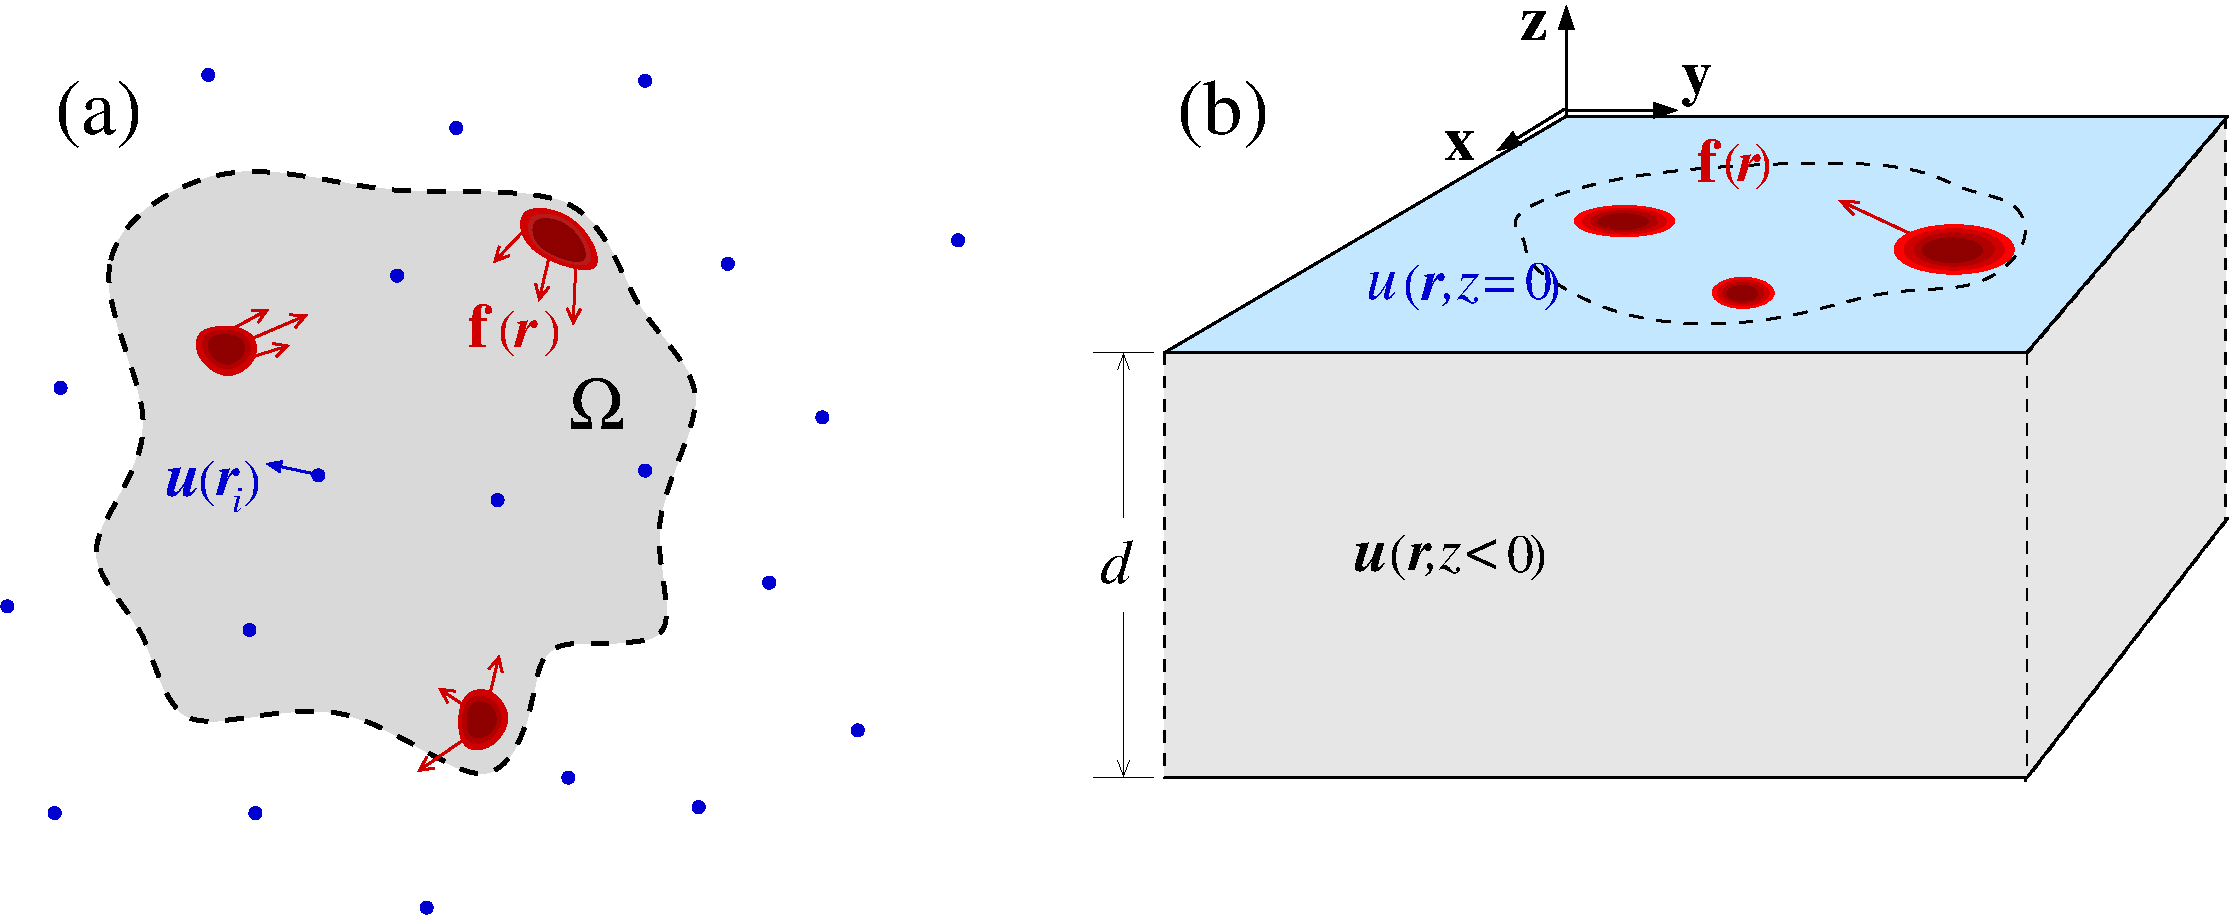
\includegraphics[width=\linewidth]{Fig1}
\caption{A schematic of an isolated cell. (a) The boundary of the cell
  footprint is denoted by the dashed curve, the support of the stress field is
  represented by the red regions that impart a stress ${\bf F}(x,y)$
  on the surface. Displacements ${\bf u}(\r_{i})$ of the elastic
  medium are measured at position $\r_{i} =
  x_{i}\hat{x}+y_{i}\hat{y}+z_{i}\hat{z}$ (blue dots) that can be
  inside or outside the cell footprint, on the surface ($z_{i}=0$), or
  below the surface ($z_{i}<0$). (b). A perspective view of the
  elastic substrate and cellular footprint.}
\label{FIG1}
\end{center}
\end{figure}

Dynamically varying force-generating structures are often small and
difficult to image, especially without biochemical modification such
as incorporation of fluorescent dyes. Therefore, other methods for
inferring their positions and magnitudes have been developed. The
simplest method relies on measuring the displacement of fiduciary
markers, such as gold nanoparticles, embedded in the elastic
substrate~\cite{WANG2007}. The measured displacements are an
indirect probe of the force-generating structures, \textit{e.g.},
focal adhesions.  Any inversion method should be able to not only
reconstruct the positions and magnitudes of the stress field, but
should ideally be able to capture potentially sharp boundaries of the
stress-generating structures.

We develop a novel method for elastic stress source recovery
using ideas developed for image segmentation.  This class of methods
relies on optimization that uses an $L^{1}$ regularization term in the
objective function.  This type of regularization term is not derived
from a fundamental physical law, but represents a prior knowledge that
the function to be recovered is sparse in content except near
edges. In addition, the overall objective function will be constructed to obey
physical constraints and symmetries.

In the next section, we review the standard linear equations of
elasticity that describe the displacement field as a function of an
arbitrary surface stress distribution. This model is then used to
construct the data mismatch term in the objective function. We then
motivate regularization and constraint terms in the full
objective function. Finally, we demonstrate our method
using both simulated and experimental data. Our method provides
good reconstruction of localized structures that exhibit desirable
qualities such as the suppression of Gibbs ringing phenomenon at the
boundaries of the stress structures.


\section{Elastic Model}

We first derive the linear elastic green's function associated with a
point force applied to the surface of a semi-infinite half-space, as
shown in Fig.~\ref{FIG1}(b). We assume that the elastic medium is
infinite in both depth ($d\to \infty$) and lateral extent. The Green's
function tensor defined in the domain ${\cal D}=\left\{(x,y,z)|x,y\in
R,z\leq0\right\}$ is given by
\begin{equation}
{\bf G^0} = \left[ \begin{matrix} G^0_{xx}(x,y,z) & G^0_{xy}(x,y,z) & G^0_{xz}(x,y,z) \\
	G^0_{yx}(x,y,z) & G^0_{xy}(x,y,z) & G^0_{yz}(x,y,z) \\
	G^0_{zx}(x,y,z) & G^0_{zy}(x,y,z) & G^0_{zz}(x,y,z) 
 \end{matrix} \right]
\end{equation}
where the components are explicitly \cite{LANDAU}
%
\begin{align}
\lefteqn{G^0_{ss}(x,y,z) = }\nonumber\\
&\frac{1+\nu}{2\pi E}\left[\frac{2(1-\nu)R_{\perp}-z}{R_{\perp}(R_{\perp}-z)} + 
\frac{[2R_{\perp}(\nu R_{\perp}-z)+z^{2}]s^{2}}{R_{\perp}^{3}(R_{\perp}-z)^{2}}\right],
\end{align}
%\begin{equation}
%G_{yy} =\frac{1+\nu}{2\pi E}\left[\frac{2(1-\nu)R_{\perp}-z}{R_{\perp}(R_{\perp}-z)}
%+\frac{[2R_{\perp}(\nu R_{\perp}-z)+z^{2}]y^{2}}{R_{\perp}^{3}(R_{\perp}-z)^{2}}\right],
%\end{equation}
\begin{equation}
G^0_{zz}(x,y,z) =\frac{1+\nu}{2\pi E}\left(\frac{2(1-\nu)}{R_{\perp}}+\frac{z^{2}}{R_{\perp}^{3}}\right),
\label{eq:Gzz0}
\end{equation}
\begin{equation} 
G^0_{xy}(x,y,z) = G_{yx}=\frac{1+\nu}{2\pi E}\frac{[2R_{\perp}(\nu R_{\perp}-z)+z^{2}]xy}{R_{\perp}^{3}
(R_{\perp}-z)^{2}},
\label{eq:Gxy0}
\end{equation}
\begin{equation}
G^0_{sz, zs}(x,y,z) =\frac{1+\nu}{2\pi E}\left(\frac{sz}{R_{\perp}^{3}}\pm\frac{(1-2\nu)s}{R_{\perp}
(R_{\perp}-z)}\right).
\end{equation}
%
and $s\equiv x,y$. The equation with $\pm$ corresponds to $G^0_{sz}$
and $G^0_{zs}$, respectively, and $R_{\perp} \equiv \sqrt{x^{2}
  +y^{2}}$. The Young's modulus and Poisson ratio of the elastic
substrate are denoted by $E$ and $\nu$, respectively.  The
displacement of a material point at $(x,y,z\leq 0)$ in the medium due
to a stress distribution ${\bf F}$ is simply the convolution $\u(\r)
\equiv [u_x \ u_y\ u_z]^\intercal = {\bf G^0}\Conv\F$.



%, while for a surface-localized force distribution, 
%$\F=(F_{x}(x,y,z=0),F_{y}(x,y,z=0),F_{z}(x,y,z=0))$ the displacement would be

%\begin{equation}
%\left[\begin{array}{c} u_{x}\\u_{y}\\u_{z}\end{array}\right]=
%\left[\begin{array}{ccc} G_{xx}&G_{xy}&G_{xz}\\G_{yx}&G_{yy}&G_{yz}\\G_{zx}&G_{zy}&G_{zz}
%\end{array}\right]
%\left[\begin{array}{c} F_{x}\\F_{y}\\F_{z}\end{array}\right]
%\end{equation}
%
%
%For a force distributation
%
%\begin{equation}
%\F=(F_{x}(x,y),F_{y}(x,y),F_{z}(x,y)) 
%\end{equation}
% 
%exerting on the surface of the medium,the displacement would be:

%\begin{equation}
%u_{i}(\r) = \int \dd \r_{\perp}'\dd z'
%G_{ij}(\r_{\perp}-\r_{\perp}',z-z')
%F_{j}(\r_{\perp}', z'),
%\label{UMODEL0}
%\end{equation}
% 
%where $\r = (\r_{\perp},z)$, $\r_{\perp}=x\hat{x} + y\hat{y}$ and
%$\r_{\perp}'= x'\hat{x} + y'\hat{y}$.  We will use this expression for
%the displacement as the model for the data term in the objective
%function for our inverse problem.

For our specific problem, we shall restrict the forces to surface
stresses $\sigma_{x,y}$ that act on the plane perpendicular to the
$\hat{z}$ axis. We define the in-plane stress distribution, at depth $z$, as
$\bs(x,y,z) = \sigma_{xz}(x,y,z)\hat{x} + \sigma_{yz}(x,y,z)\hat{y}$. 
The resulting surface-level displacement fields become

\begin{align}
u_{x}(x,y) &= \int_\Omega \dd x'\dd y'G_{xx}(x-x',y-y')\sigma_{xz}(x',y') \nonumber\\
&\qquad +  \int_\Omega \dd x'\dd y'G_{xy}(x-x',y-y')\sigma_{yz}(x',y') \label{eq:UMODEL1x}  \\
u_y(x,y) &= \int_\Omega \dd x'\dd y'G_{yx}(x-x',y-y')\sigma_{xz}(x',y') \nonumber\\
&\qquad +  \int_\Omega \dd x'\dd y'G_{yy}(x-x',y-y')\sigma_{yz}(x',y'),  \label{eq:UMODEL1y}  
\end{align}
%
where

\begin{equation}
G_{\cdot,\cdot}(x,y) = G^0_{\cdot,\cdot}(x,y,z=0),
\end{equation}
%
and by abuse of notation,

\begin{equation}
\sigma_{xz}(x,y) = \sigma_{xz}(x,y,z=0) \quad \sigma_{yz}(x,y) =
\sigma_{yz}(x,y,z=0).
\end{equation}
Note that tangential stresses can lead to displacement in the normal direction.

%

\section{Inverse problem}

Here, we develop an objective function for which the minimizing
solution provides a good approximation to the underlying stress field,
while preserving discontinuities.  The first component is simply a
quadratic data mismatch term defined by the sum over the displacements
measured at the $N$ measurement positions at $\r_{i}$:

\begin{equation}
\Phi_{\rm data}[\bs] = \sum_{i}^{N}\vert \u^{\rm
  data}(\r_{i})- \u(\r_i)\vert^{2}.
\end{equation}
%
Since $\u^{\rm data}(\r_{i})$ is given, and $\u(\r_{i})$, is given by
Eqs.~\ref{eq:UMODEL1x} and~\ref{eq:UMODEL1y}, this contribution to the
objective function is a functional over the surface-stress function
$\bs(\r_{\perp})$.  For simplicity, we will assume that the data
points are sampled over an uniform grid with coordinates given $\{
(x_j,y_k) : j\in\{1,2,\ldots,J\}, k\in\{1,2,\ldots,K\}\}.$

In Eqs~\ref{eq:UMODEL1x} and~\ref{eq:UMODEL1y}, we have restricted the
domain of integration to lie within the cell footprint $\Omega$,
futher emphasizing that $\boldsymbol\sigma$ has compact support. As a
consequence of compact support, for a fixed, discretized approximation
of $\sigma_{xz},\sigma_{yz}$, the displacements can be obtained
exactly by solving an equivalent system of linear equations of finite
dimension.

Here we explicitly define this system of linear equations given a
piecewise-affine approximation of the stress field. Let us consider
the first-order approximation of $\sigma_{xz}$ and $\sigma_{yz}$ using
central finite differences, for $x\in[x_j - \delta x/2, x_j+\delta
  x/2) \cap y\in[y_j-\delta y/2, y_j + \delta y /2)$,
\begin{align}
\lefteqn{\sigma_{xz}(x,y) =\sigma_{xz}(x_i , y_j)  }\nonumber \\
& \qquad+ (x-x_i)\frac{\sigma_{xz}(x_{i+1},y_j) -\sigma_{xz}(x_{i-1},y_j) }{2\delta x}  \nonumber\\
&\qquad + (y-y_j)\frac{\sigma_{xz}(x_i,y_{j+1}) - \sigma_{xz}(x_i,y_{j-1}) }{2\delta y} \nonumber\\
&\qquad + \mathcal{O}(\delta x)^2 + \mathcal{O}(\delta y)^2,\label{eq:sigma_affine}
\end{align}
where $i,j$ denotes a tuple of grid coordinates. In effect, we are
performing sub-pixel interpolation of the stress where the stress is
fully-determined by its values at the grid vertices.

We may now rewrite Eq.~\ref{eq:UMODEL1x}, for instance, to solve for
the displacement at a location $(x_n,y_m)$, by decomposing the
integral into a sum of integrals over grid cells
%
\begin{widetext}
\begin{align}
 \lefteqn{u_x(x_n,y_m) =} \nonumber\\
 & \sum_{(x_j,y_k)\in\Omega} \Bigg\{ \Bigg[\sigma_{xz}(x_j,y_k)  - x_j\left(\frac{\sigma_{xz}(x_{j+1},y_k) - \sigma_{xz}(x_{j-1},y_k) }{2\delta x }    \right)    -y_k\left( \frac{\sigma_{xz}(x_j,y_{k+1}) -  \sigma_{xz}(x_j,y_{k-1}) }{2\delta y}\right) \Bigg]{ \langle G_{xx} \rangle}^{nmjk} \nonumber \\
&\quad+\left[ \frac{\sigma_{xz}(x_{j+1},y_k) -  \sigma_{xz}(x_{j-1},y_k) }{2\delta x}   \right]\langle xG_{xx} \rangle^{nmjk} + \left[  \frac{\sigma_{xz}(x_j,y_{k+1}) - \sigma_{xz}(x_j,y_{k-1}) }{2\delta y} \right] \langle yG_{xx} \rangle^{nmjk}\nonumber\\
&\quad+  \Bigg[\sigma_{yz}(x_j,y_k) -x_j\left(\frac{\sigma_{yz}(x_{j+1},y_k) - \sigma_{yz}(x_{j-1},y_k) }{2\delta x}    \right)    -y_k\left( \frac{\sigma_{yz}(x_j,y_{k+1}) - \sigma_{yz}(x_j,y_{k-1}) }{2\delta y}\right) \Bigg] \langle G_{xy} \rangle^{nmjk}\nonumber \\
&\qquad +\left[ \frac{\sigma_{yz}(x_{j+1},y_k) -  \sigma_{yz}(x_{j-1},y_k) }{2\delta x}   \right]  \int_{y_k-\delta y/2}^{y_k+\delta y/2}  \langle xG_{xy} \rangle^{nmjk} + \left[  \frac{\sigma_{yz}(x_j,y_{k+1}) - \sigma_{yz}(x_j,y_{k-1}) }{2\delta y} \right] \langle yG_{xy} \rangle^{nmjk} \Bigg\},
\label{eq:ux_decomposed}
\end{align}
\end{widetext}
%
where

\begin{align}
%\lefteqn{\langle G_{st} \rangle^{nmjk} = }\nonumber\\
%&\qquad    \int_{y_k-\delta y/2}^{y_k+\delta y/2} \int_{x_j-\delta x/2}^{x_j+\delta x/2} G_{st}(x_n-x',y_m-y') \dd x' \dd y' \label{eq:G_ave} \\
\lefteqn{\langle g(x,y)G_{st} \rangle^{nmjk} =}  \nonumber\\
&\  \int_{y_k-\delta y/2}^{y_k+\delta y/2} \int_{x_j-\delta x/2}^{x_j+\delta x/2} g(x',y')G_{st}(x_n-x',y_m-y') \dd x' \dd y', \label{eq:G_ave} 
\end{align}
%
except that at the edges where we use one-sided differences so that we
are only differentiating within $\Omega$. Explicit closed-form
expressions for the integrals represented by Eq.~\ref{eq:G_ave2} are
given in the Supplemental Materials. A similar expression can be found
for solving for $u_y$ (not shown).

Regrouping terms, we can now define the linear system of equations for
solving for $u_x$ at all grid points simultaneously,
\begin{equation}
u_x^{nm} = X^{nmjk}\sigma_{xz}(x_j,y_k) + Y^{nmjk}\sigma_{yz}(x_j,y_k),
\label{eq:linearsystem1}
\end{equation}
where summation is implied over each index tuple $(j,k)$, and the
coefficient matrices are defined as
\begin{align}
\lefteqn{X^{nmjk} = \langle G_{xx} \rangle^{nmjk} -  \langle G_{xx} \rangle^{n,m,j-1,k}\frac{x_{j-1}}{2\delta x} } \nonumber\\
&\quad  + \langle G_{xx} \rangle^{n,m,j+1,k}\frac{x_{j+1}}{2\delta x} -  \langle G_{xx} \rangle^{n,m,j,k-1}\frac{y_{k-1}}{2\delta y}  \nonumber\\
&\quad + \langle G_{xx} \rangle^{n,m,j,k+1}\frac{y_{k+1}}{2\delta y} -\frac{\langle xG_{xx} \rangle^{n,m,j-1,k}}{2\delta x}  \nonumber\\
&\quad +\frac{\langle xG_{xx} \rangle^{n,m,j+1,k}}{2\delta x} - \frac{\langle yG_{xx} \rangle^{n,m,j,k-1}}{2\delta y} \nonumber\\
&\quad+\frac{\langle yG_{xx} \rangle^{n,m,j,k+1}}{2\delta y} \label{eq:linearsystemX}
\end{align}
\begin{align}
\lefteqn{ Y^{n,m,j,k} =  \langle G_{xy} \rangle^{nmjk} - \langle G_{xy} \rangle^{n,m,j-1,k}\frac{x_{j-1}}{2\delta x} } \nonumber\\
&\quad+\langle G_{xy} \rangle^{n,m,j+1,k}\frac{x_{j+1}}{2\delta x} - \langle G_{xy} \rangle^{n,m,j,k-1}\frac{y_{k-1}}{2\delta y} \nonumber\\
&\quad+\langle G_{xy} \rangle^{n,m,j,k+1}\frac{y_{k+1}}{2\delta y}  -\frac{\langle xG_{xy} \rangle^{n,m,j-1,k}}{2\delta x} \nonumber \\
&\quad +\frac{\langle xG_{xy} \rangle^{n,m,j+1,k}}{2\delta x} - \frac{\langle yG_{xy} \rangle^{n,m,j,k-1}}{2\delta y} \nonumber\\
 &\quad+\frac{\langle yG_{xy} \rangle^{n,m,j,k+1}}{2\delta y}.\label{eq:linearsystemY}
\end{align}

From the equation-counting perspective, the system of equations is
exactly determined given that one has at least as many measurement
points as grid cells in the resolution that one wishes to reconstruct
the stress field, provided that one is able to measure displacements
in both principle directions. Even if one is able to measure both
displacements, the problem may still be highly ill-conditioned since
measurements are taken in the presence of noise at a finite
precision. To resolve these issues, we introduce the concept of
physically consistent regularization as applied to this problem.

\subsection{Physical regularization}

So far, the construction of the surface stress, even at the finite
resolution where measurements are available, is ill-conditioned. We
regularize this problem, by forcing the reconstruction to obey some
physically-relevant characteristics of the surface stress. First,
since we are assuming inertial effects are negligible, we require that
the net force is zero, or that
\begin{equation}
\int_\Omega\sigma_{xz}(x,y)\dd x \dd y= \int_\Omega\sigma_{yz}(x,y)\dd x \dd y = 0 .
\end{equation}
Likewise, we require that there is no net torque, or that
\begin{equation}
\int_\Omega\sigma_{yz}(x,y)x \dd x \dd y  = \int_\Omega\sigma_{xz}(x,y)y \dd x \dd y .
\end{equation}
%
Finally, we would like to impose regularity on the reconstructed
fields while preserving both rotational invariance and the sharp
stress boundaries. To this end we employ a variant of a penalty used often in
image processing applications, where we wish to penalize the $L^1$
norm of the variation in the fields, or the total variation. To do
this in a manner that is consistent with the philosophy that
rotation of the data should not affect the result, we penalize the
total variation norm of the invariants of the stress tensor. In the
case of two-dimensional tensors, of which the surface stress is an
example, the tensor invariants are the trace
\begin{equation}
\textrm{Tr}(\bsigma) = \sigma_{xz} + \sigma_{yz}
\end{equation}
and the determinant
\begin{equation}
\textrm{Det}(\bsigma) = \sigma_{xz} \sigma_{yz}.
\end{equation}
Any regularization penalty imposed on the reconstruction problem must
be a functional of these invariants in order to maintain rotational
invariance, relative to the choice of observation frame, of the
reconstructed stress tensor.
 
For this manuscript, we investigate penalty functionals on the trace
of the stress tensor. In particular, we are interested in the $L^1$
norm of the trace
\begin{equation}
\Phi_{L^1(Tr)} = \int_\Omega \vert \sigma_{xz}(x,y) + \sigma_{yz}(x,y)  \vert \dd x\dd y
\label{eq:PhiL1Tr}
\end{equation}
and total variation norm of the trace
%
\begin{equation}
\Phi_{TV(Tr)} =  \int_\Omega | \nabla(\sigma_{xz}(x,y) + \sigma_{yz}(x,y) ) | \dd x\dd y.
\label{eq:PhiTVTr}
\end{equation}

Using either of these expressions as the regularization norm
$\Phi_{\textrm{reg}}$ suggests the penalized optimization problem

\begin{equation}
\hat{\bsigma} \big\vert \lambda = \arg\min_{\bsigma} \left\{ \Phi_{\textrm{data}}[\bsigma] + 
\lambda\Phi_{\textrm{reg}}[\bsigma] \right\},\label{eq:objective}
\end{equation}
subject to the no-force and no-torque constraints mentioned above,
where $\lambda>0$ is a tunable parameter. This problem is in a
standard form that is directly solvable using a variety of
optimization routines.  In our implementation, we use a second-order
quadratic cone solver.

\subsection{Reducing computation by using a cut-off}
To reduce the size of the system of equations described in
Eqs.~\ref{eq:linearsystem1}--\ref{eq:linearsystemY}, we note that the
Green's function falls off at a rate of $|\r|^{-1}$. However, when
combined with the zero-force constraint, the relationship between the
displacements and the support of the stress field falls off at the
much quicker rate of $|r|^{-2},$ under a set of reasonable assumptions
that are consistent with the choice of regularization that we have
made.

\begin{lem} 
      \label{lem:multipole}
Let $\Omega = supp(\bsigma)\subset \mathbb{R}^2$ be compact, and
assume that $\bsigma\in L^1(\Omega)$. For a fixed
$\mathbf{x}\not\in\Omega$, denote $D(\mathbf{x}) = \inf\{ ||
\mathbf{x} -\mathbf{y}|| : \mathbf{y}\in\Omega \}$. Then, for
$\mathbf{x}$ where $D(\mathbf{x})\geq R>0$,
\begin{equation}
\vert u_x(\mathbf{x}) \vert \leq \frac{C_x\norm{\bsigma}_1}{R^2}
\end{equation}      
and
\begin{equation}
\vert u_y(\mathbf{x}) \vert \leq \frac{C_x\norm{\bsigma}_1}{R^2}
\end{equation}      
for some constants $C_x,C_y$.
\end{lem}

\begin{lem}
\label{lem:affine_error}
Let $\tilde{\bsigma}$ be an affine approximation to $\bsigma\in
C^s(\Omega)$ for $s\in\mathbb{Z}^+$, and $\tilde{\u}$ be the
corresponding displacement field completed from the approximate stress
field. Then,
\begin{equation}
\vert \tilde{\u}  - \u \vert \leq C (\delta x)^2
\end{equation}
\end{lem}

The decay of the influence of stress on the system provides
justification for setting distance-based cut-offs of the linear
system. The effect of the cut-off is to limit the left-hand side of
Eq.~\ref{eq:linearsystem1} to only locations within some maximal
distance $R$ from the outline of the cell.  The error in the solution
of the inverse problem is dependent on the precision of the
observations, the physical constants that describe the medium, and the
maximum magnitude of the stress.

\begin{thm}
\label{thm:main}
Denote $\varepsilon^R(\r) = \hat{\bsigma}^R(\r) - \bsigma(\r)$ for
$\r\in\Omega$, where $\sigma_{xz}\in L^1(\Omega)$, and
$\hat{\bsigma}^R(\r)$ is the reconstructed stress field found by
solving the optimization problem of Eq.~\ref{eq:objective} using only
the displacement data within a maximal distance of $R$ from the
cell. Then,
\begin{equation}
\sup \vert \hat{\bsigma}^R(\r) - \hat{\bsigma}^\infty(\r) \vert \leq \frac{C}{R^2}
\end{equation}

\begin{proof}
TODO... result needs refinement
\end{proof}

\end{thm}


\section{Results}

We implemented our regularized inversion method in Python version 3.5,
where optimization is performed using the \texttt{cvxpy} package with
the \texttt{ecos} solver.  Our implementation is available at
\url{https://github.com/joshchang/tractionforce}. 

First we tested our method on simulated data consisting of two different force- and
torque-free test stress fields. The first test stress field we consider is 

\begin{equation}
\sigma_{rz}(r,\theta) = f_{r} \sin (m\theta)\quad \sigma_{\theta z}(r,\theta) = f_{\theta} \cos (n\theta),
\end{equation}
%
for $a < r < 1$, and zero otherwise. Here, $m,n$ are integers and if
we normalize the stresses by the Young's modulus $E$, $f_{r}$ and
$f_{\theta}$ are constants.  

The second stress field we test consists of four separated circular
stress pads, or focal adhesions, with radii $r_{1} = 1/5$, $r_{2} =
1/6$, $r_{3} = 1/8$, and $r_{4} = 1/4$, and centers at positions
$(x_{1},y_{1}) = (-1,-1/2)$, $(x_{2},y_{2}) = (-5/4,0)$,
$(x_{3},y_{3}) = (2,1)$, and $(x_{4},y_{4}) = (0,1)$.  The pads $1,2$,
and 4 are connected as shown, while pad 3 is connected only to pad
1. The tensions along these connections give rise to surface stresses
imparted by the pads onto the substrate.  Within each of the pads,
except for pad 4, the foces will be uniformly distributed.  For pad 4,
we will assume that the filaments connecting it with pad 2 are
distributed according to a cone-like density function.  The stresses
under each patch $i$ are decomposed into contributions arising from
tensions with connected patches $j$:

\begin{align}
\sigma_{42} = -g_{42}(r)\hat{y}, \quad \sigma_{24} = \hat{y} {2\pi \over \pi r_{2}^{2}}
\int_{0}^{r_{4}}r g_{42}(r)\dd r = {3\over 4} \bar{g}_{42} \hat{y} \\
\sigma_{14} = f_{14}\hat{x} + g_{14} \hat{y}, \quad \sigma_{41} = -\left({4\over 5}\right)^{2}\sigma_{14} \\
\sigma_{12} = f_{12}\hat{x}-g_{12}\hat{y}, \quad \sigma_{21} = -\left({6\over 5}\right)^{2}\sigma_{12} \\
\sigma_{13} = f_{13}\hat{x} + g_{13}\hat{y}, \quad \sigma_{31} = -\left({8\over 5}\right)^{2}\sigma_{13}
\end{align}
%
where we have defined $\sigma_{ij}$ in units of the Young's modulus $E$ and
$f_{ij}, g_{ij} > 0$ are all dimensionless constants. The normalized 
stresses $\sigma_{ij}$ are nonzero only 
in the disk $r_{i}$. All stress distributions are constant inside 
the disks except for

\begin{equation}
g_{42}(r) = \bar{g}_{42} \left(1-{r \over r_{4}}\right),
\end{equation}
%
where $\bar{g}_{42}$ is a constant that sets the maximum value of
$g_{42}(r=0)$. The way to interpret this physically is that the
multiple filaments that connect patch 4 to patch 2 are uniformly
attached under pacth 2, but {\it not} under patch 4.  The density of
attachments linearly decrease from the center of patch 4. This
variation in attachment density arises only for those filaments that
attach patch 4 to patch 2, and only at patch 4.  The all other
filaments are assumed to attach uniformly under each pad.  In this
test case, the tension between pads 1 and 3 is $T_{13} =
(1/5)^{2}\sqrt{f_{13}^{2} + g_{13}^{2}}$. Both test fields, along with 
possible cell footprint boundaries are shown in
Fig.~\ref{TEST}. 

\begin{figure}[t]
\begin{center}
%\input{Fig1.pstex_t}
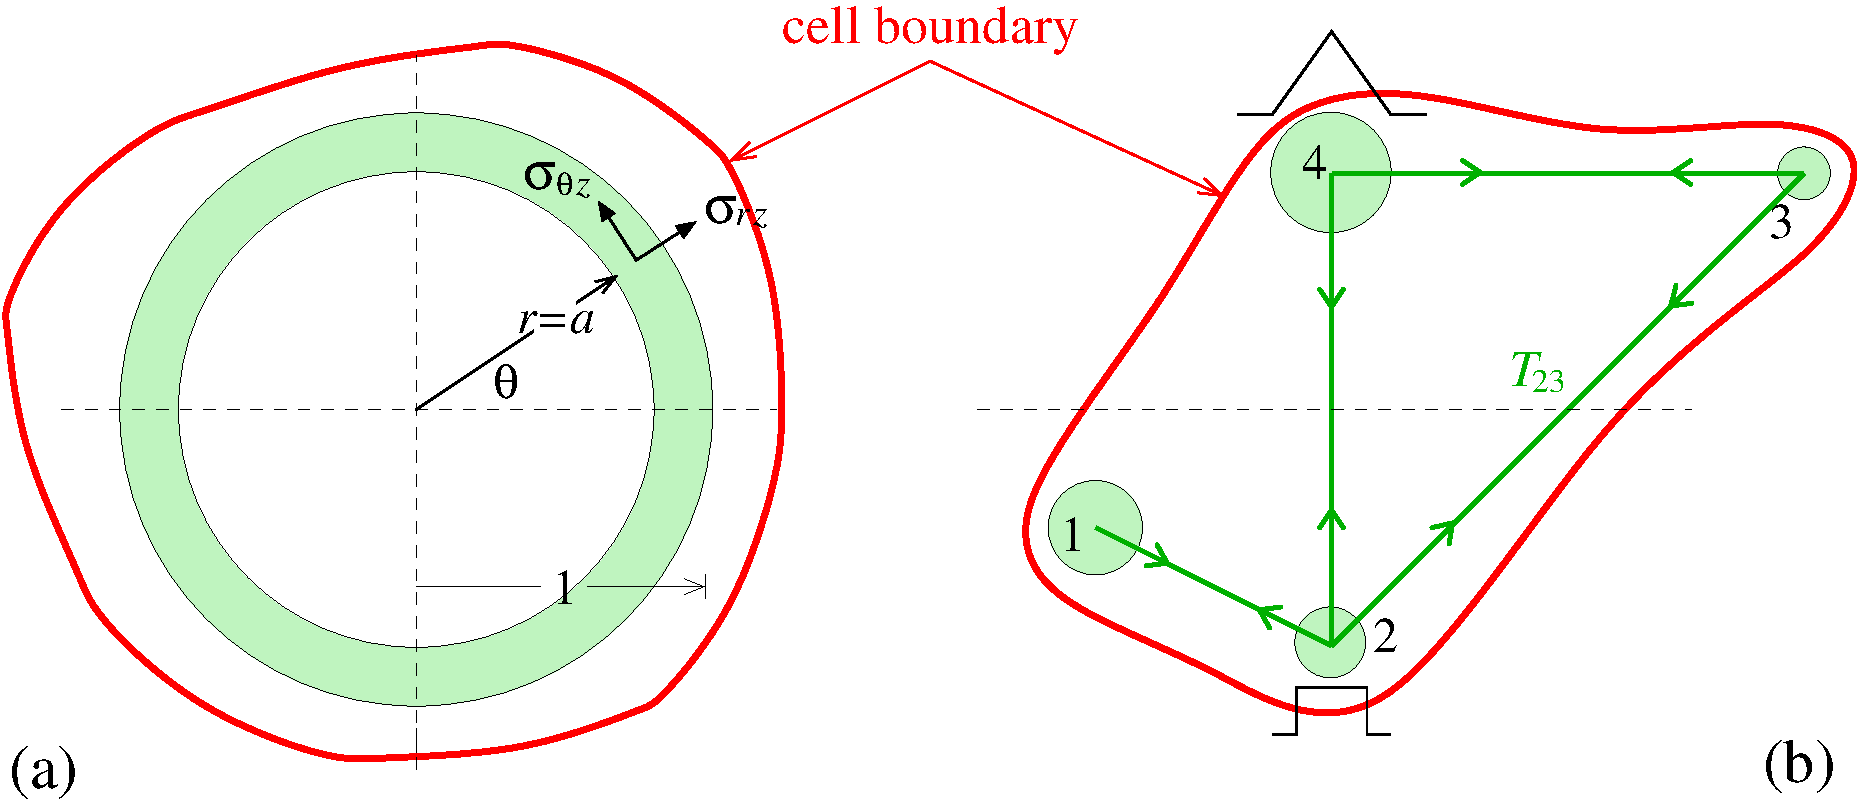
\includegraphics[width=5in]{tests.eps}
\caption{\textbf{Test stress fields.} (a) An annular stress distribution containing forces in the
  $\theta$ and $r$ directions. (b) Four focal adhesions under mutual
  tension as by the green lines representing filaments. The red
  borders represent the extent of the cell footprint and can be
  determined experimentally as part of the imaging.  Mathematically,
  the cell boundary forms the basis for a constraint on the stress
  distribution and we explore the quality of inversion depends on this
  constraint.}
\label{TEST}
\end{center}
\end{figure}


RESULTS AND PLOTS FOR TEST STRESS FIELDS:

\begin{figure}[t]
\begin{center}
%\input{Fig1.pstex_t}
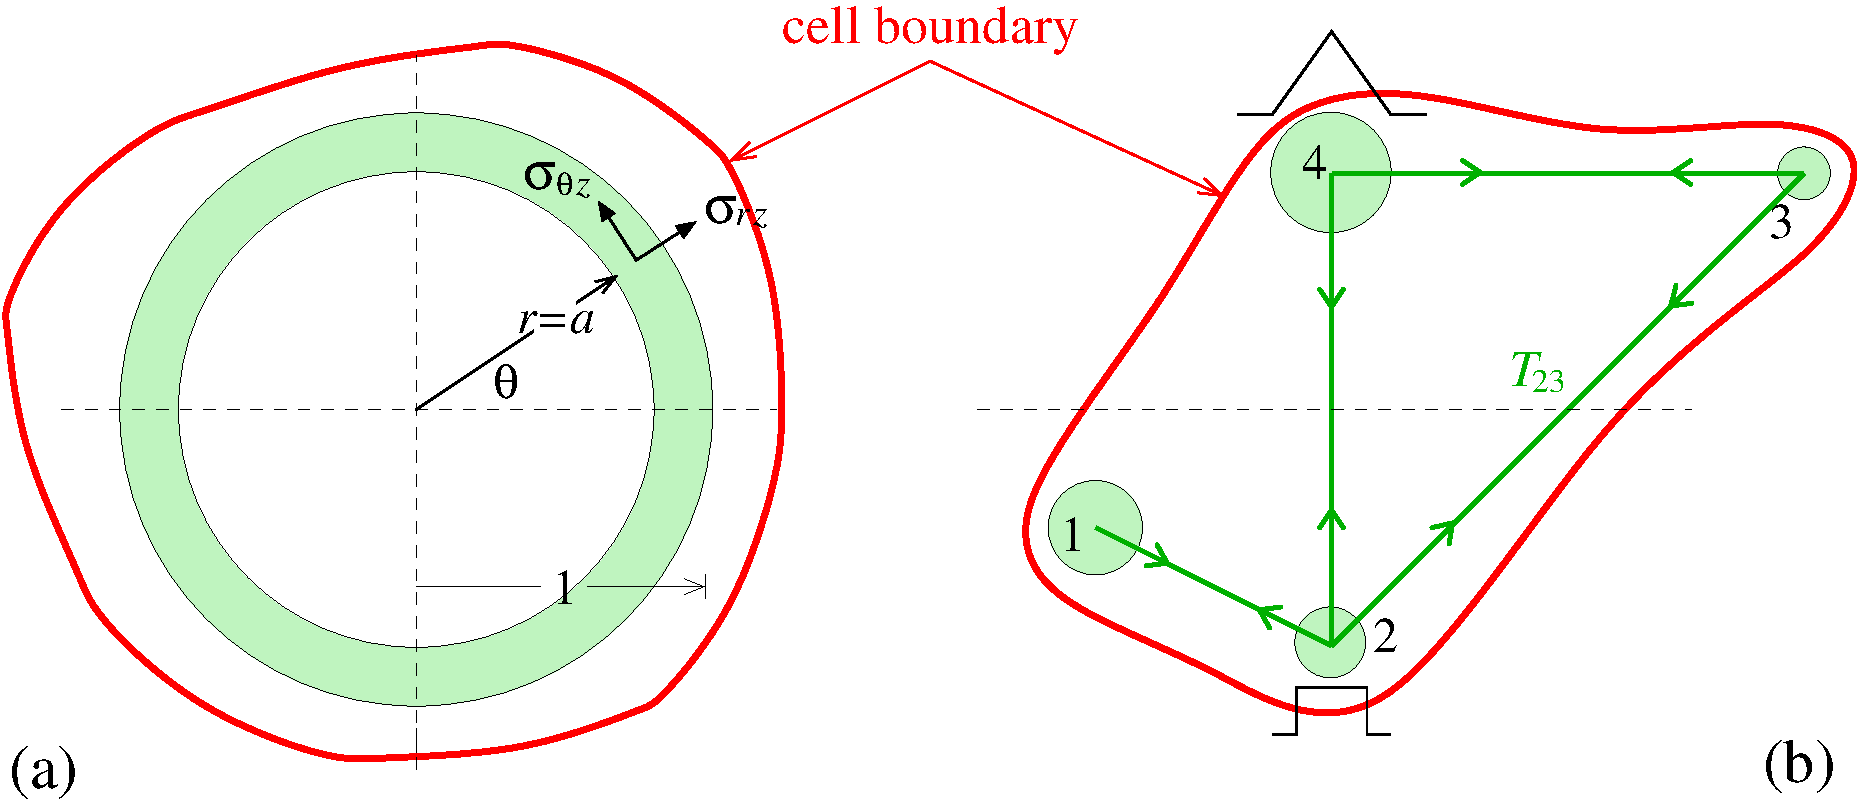
\includegraphics[width=5in]{tests.eps}
\caption{\textbf{Inversion results for test stress fields.} (a) Inversion for 
the annular stress field with $m=4$, $n=2$ and ...using different cell boundaries.... }
\label{RESULTS_TEST}
\end{center}
\end{figure}


Next, we consider experimental displacements resulting from stress
generated by a single cell. The surface displacements were measured
using Hilbert space dynamometry which uses phase information of the
periodic signal arising from a chemically patterned grid on the
substrate \cite{POPESCU}.  Both $x$ and $y$-displacements at a resolution of the
patterned grid spacing can be measured, as shown in Fig.~\ref{DATA}

\begin{figure}
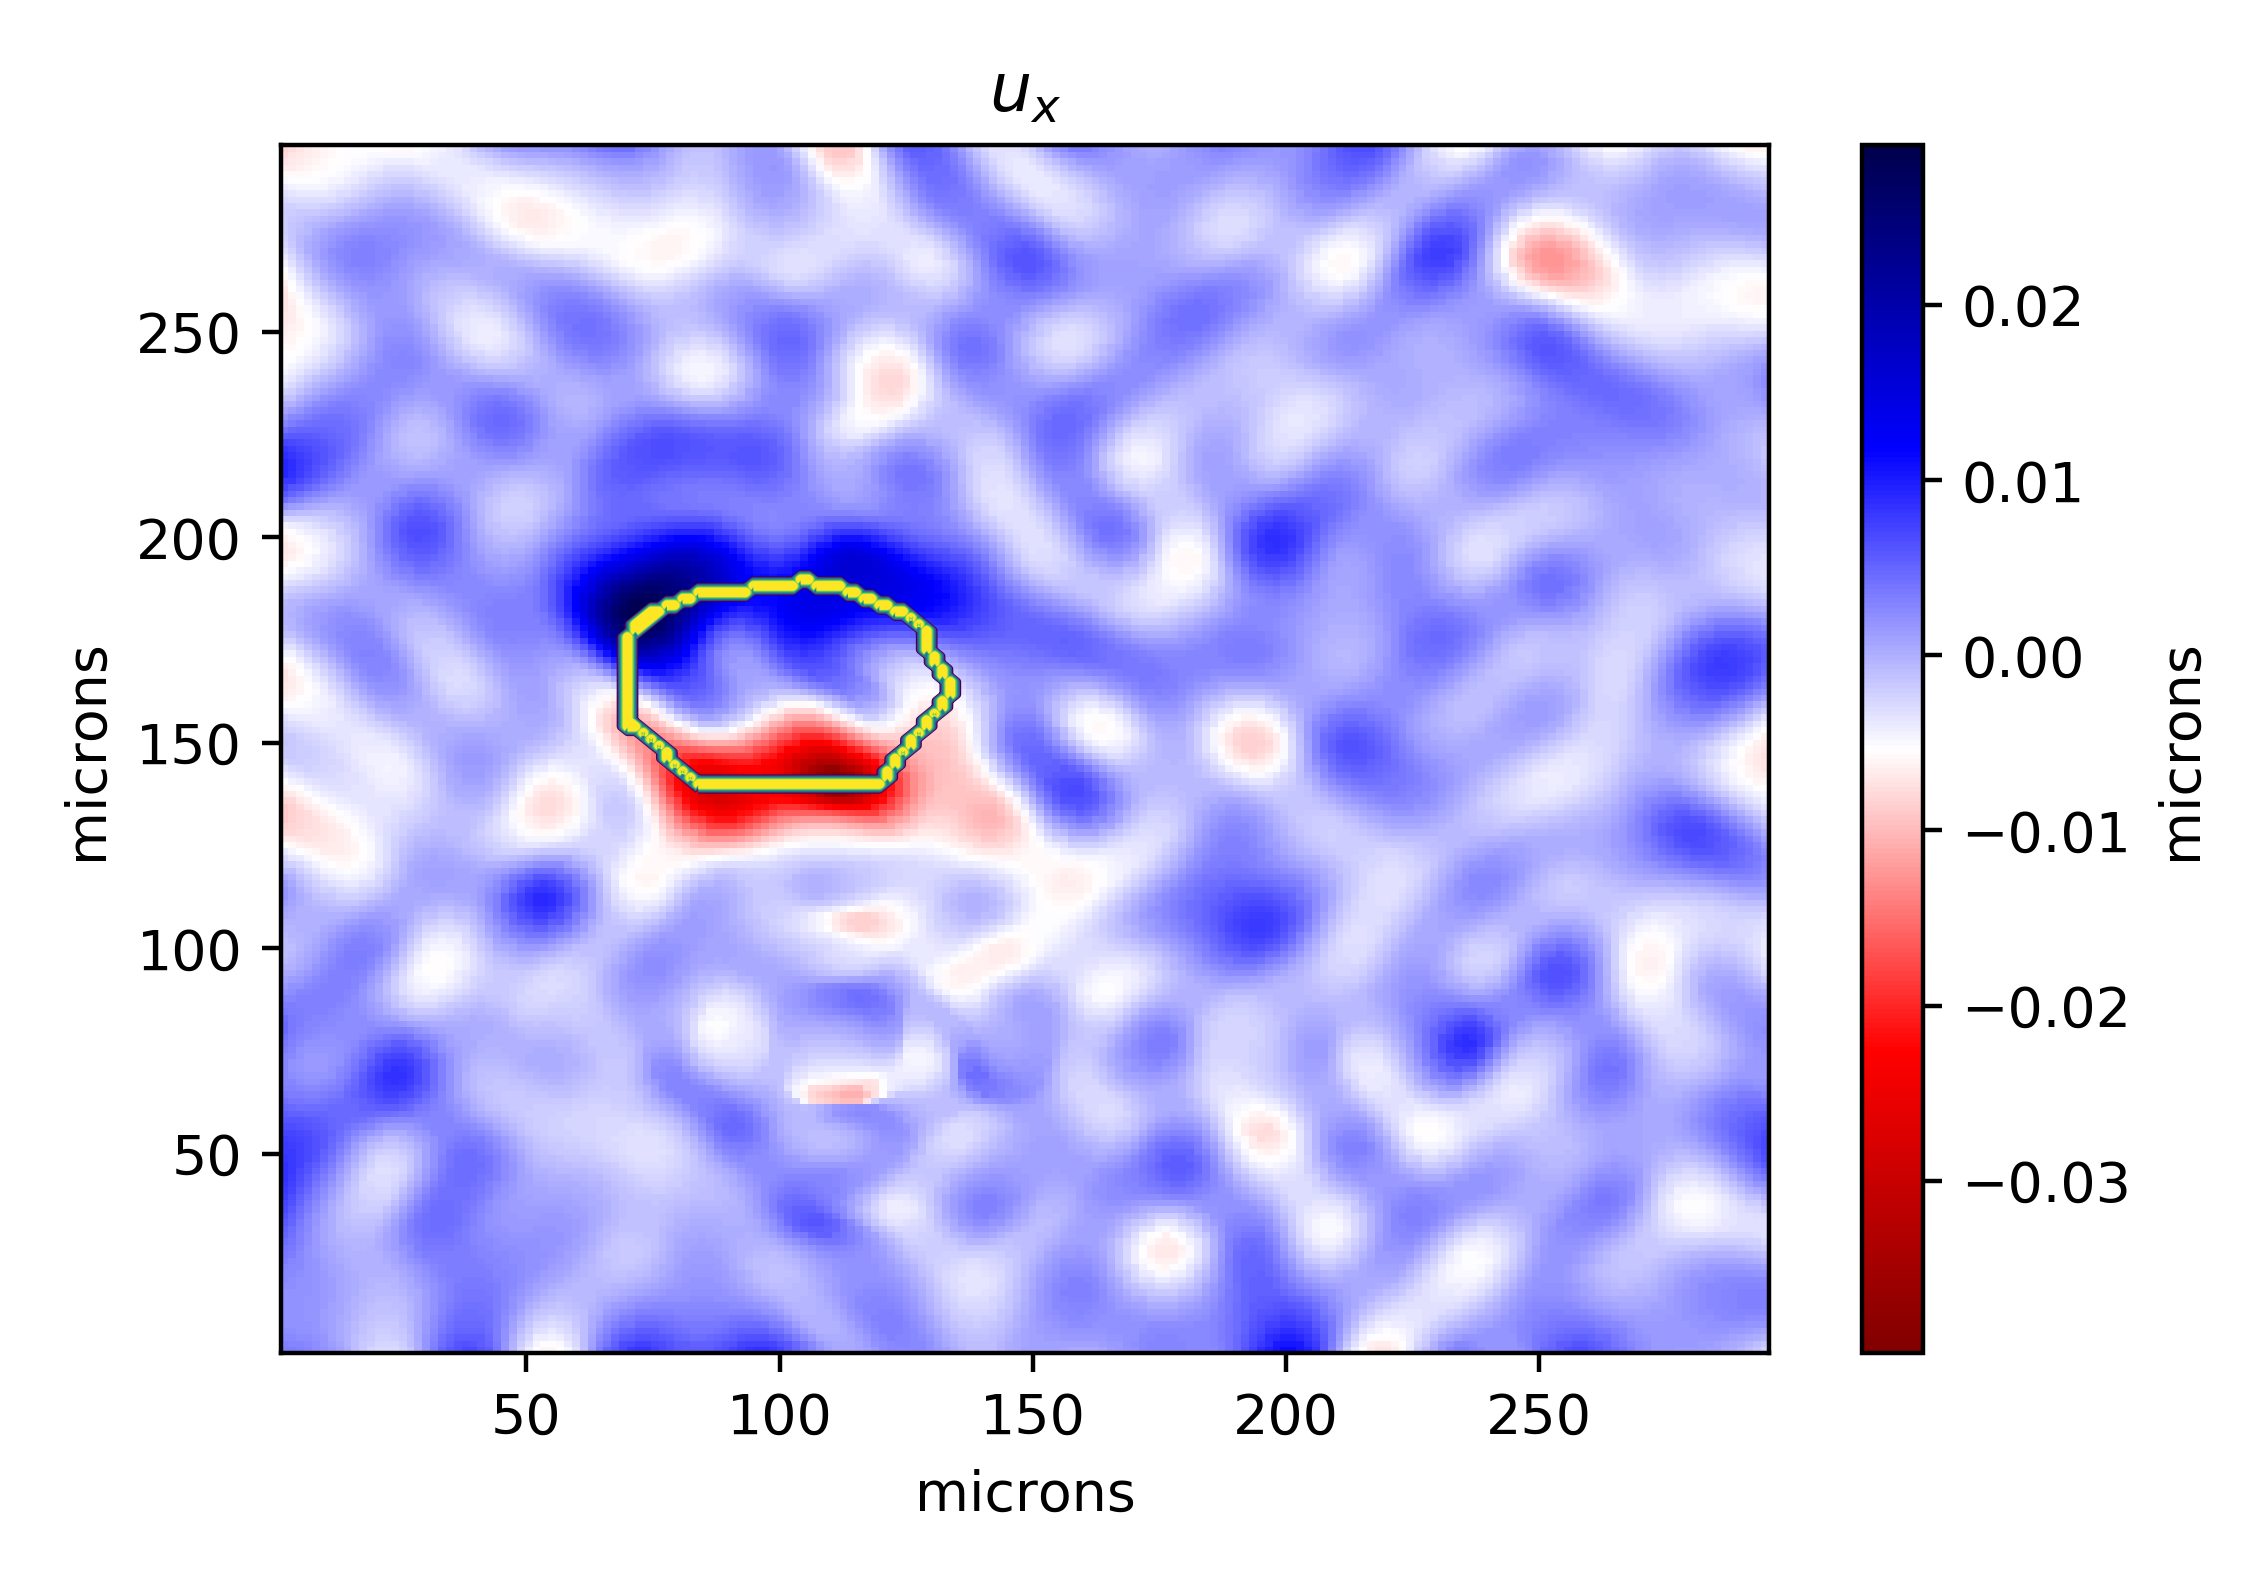
\includegraphics[width=\linewidth]{fig0a}
\caption{\textbf{Bright field image and displacements.} (a) Raw bight
  field image of a mesenchymal stem cell. The cell footprint boundary
  is estimated from segmentation. (b) and (c) The $x-$ and
  $y-$displacement fields at the surface of the substrate.}
\label{DATA}
\end{figure}
%
The results of reconstruction of the stress field using our method are
shown in Fig.~\ref{fig:fig2}.

\begin{figure*}
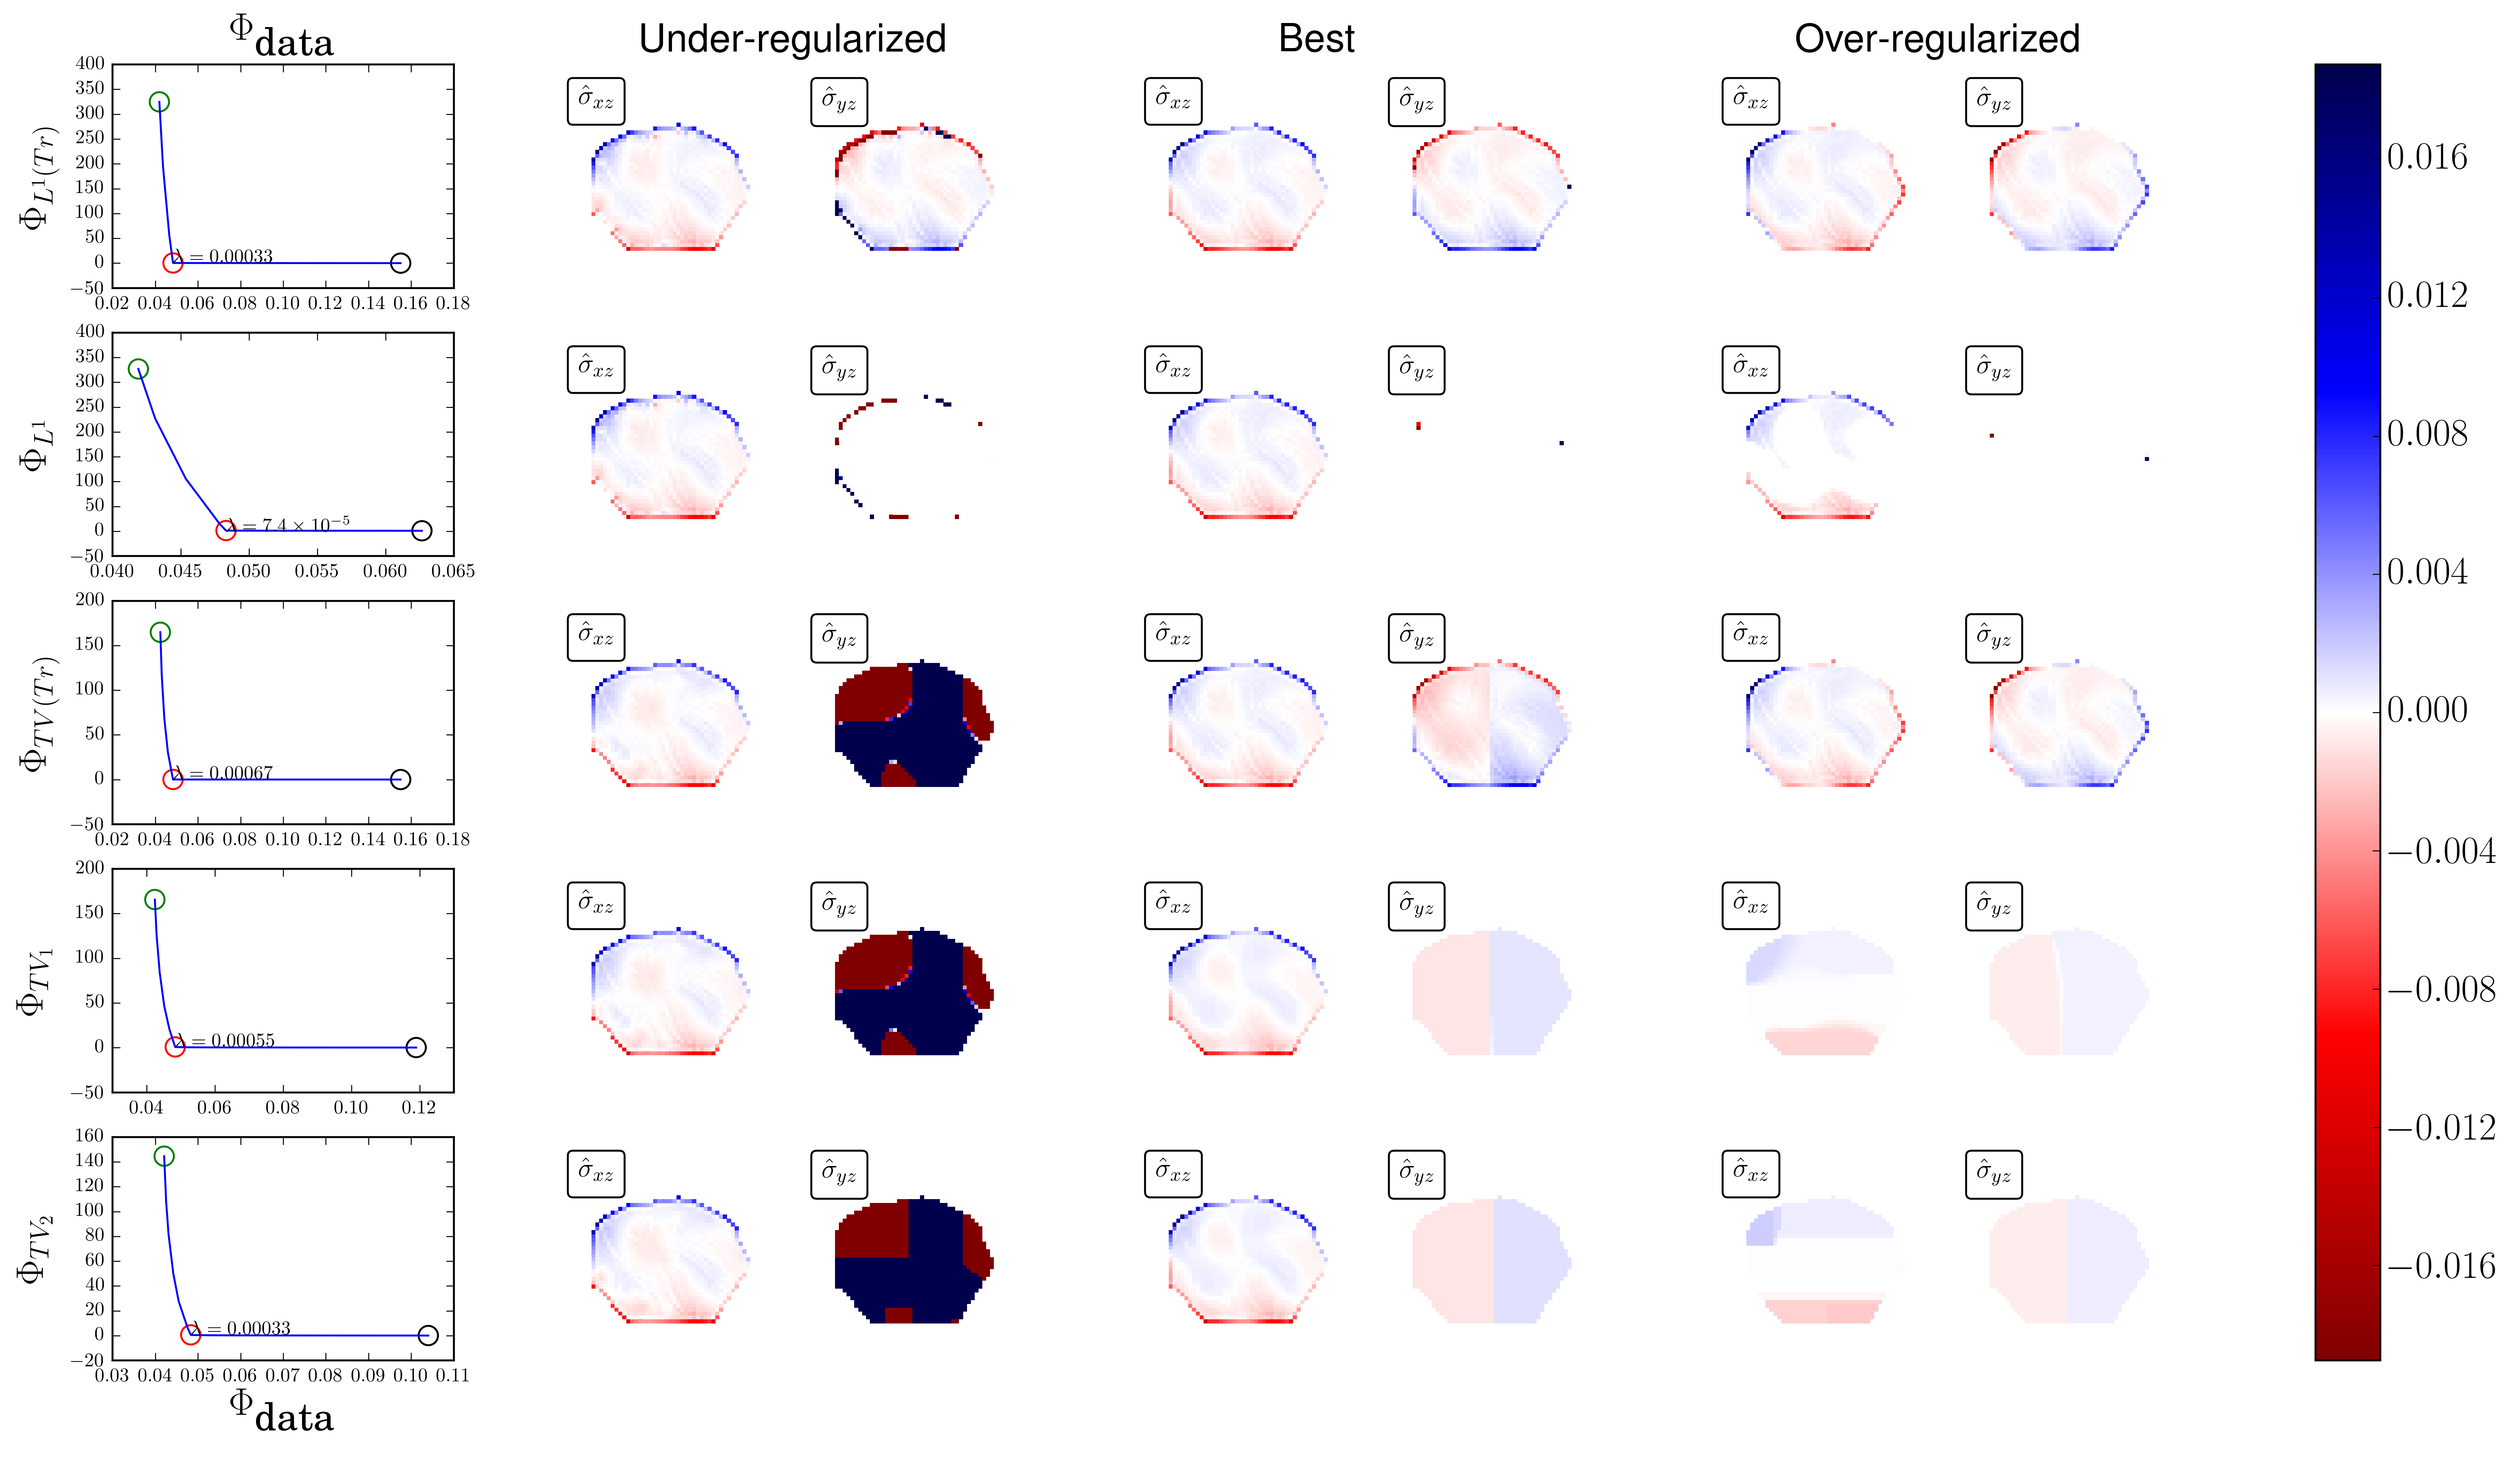
\includegraphics[width=\linewidth]{fig2}
\caption{\textbf{Reconstruction of experimental surface stress field} for various
  choices of regularization. The first and third rows are
  physically-consistent regularizations. The best reconstruction
  balances regularity and data matching and corresponds to the value
  for $\lambda$ that is near a phase transition in the trade off plot
  between these two penalties (circled in red). The under-regularized
  solution corresponds to the point circled in green and the
  over-regulated solution corresponds to the point circled in black.}
\label{fig:fig2}
\end{figure*}

We also compared reconstruction of the surface stress using our
rotationally invariant norms of Eq.~\ref{eq:PhiL1Tr} and
Eq.~\ref{eq:PhiTVTr} against alternate isotropic norms. As an
alternative to the $L^1$ norm on the trace we compared
\begin{equation}
\Phi_{L1} = \int_\Omega \left\vert \sigma_{xz}(x,y) +\sigma_{yz}(x,y) \right\vert\d\r,
\end{equation} 
and as alternatives to the total variation on the trace we looked at

\begin{equation}
 \Phi_{TV_1} = \int_\Omega \left( \vert\nabla\sigma_{xz}(x,y) \vert +
 \vert\nabla\sigma_{yz}(x,y) \vert\right)\d\r
 \label{eq:PhiTV1}
\end{equation}
and
\begin{equation}
\Phi_{TV_2} = \int_\Omega  \left( \vert\partial_x\sigma_{xz}\vert + \vert\partial_y\sigma_{xz}\vert + \vert\partial_x\sigma_{yz}\vert+ \vert\partial_y\sigma_{yz}\vert\right)\d\r.
 \label{eq:PhiTV2}
\end{equation}
%
The adjustable parameter $\lambda$ was chosen in each instance by
examining the balance between data mismatch and regularity using
trade-off curves shown in Fig.~\ref{fig:fig2}, and taking the value
for $\lambda$ that yields a point farthest away from the line segment
joining the ends of the plot. In Fig.~\ref{fig:fig2}, the chosen value
of $\lambda$ corresponds to the given balance between regularity and
data fidelity marked by the red circle. The solution corresponding to
this particular value of $\lambda$ is shown in the middle column on
the right. For reference, under-regularized solutions, corresponding
to the green circle in the trade-off plot, and over-regularized
solutions, corresponding to black circle, are also given. Each row in
Fig.~\ref{fig:fig2} corresponds to the use of a different
regularization penalty functional. In all of these reconstructions, we
have imposed that the surface stress is both force-free and torque
free, and also that the support of the stress is within given cell
boundaries.

To explore the effect of the constraints on our reconstructions, we
systematically removed them in solving the rotationally invariant
$L^1$ regularized problem In Fig.~\ref{fig:fig3}, we present
reconstructions where net torque is free to vary but force is
constrained, where net force is free to vary but torque is
constrained, and where net torque and force are both free to vary. In
each of these reconstructions the unconstrained quantity did not sum
to zero, as desired.

Additionally, our reconstructions are implicitly constrained by the
assumption of compact support where the support of the stress tensor
is within the cell boundary. Examining Fig.~\ref{fig:fig2}, it appears
that this constraint is active as much of the stress is concentrated
at boundaries. In Fig.~\ref{fig:fig4}, we loosened the boundary
constraint by allowing the support of the stress to fall within 10
pixels of the cell boundary.


APPLY THESE LAST TWO ANALYSES TO TEST DATA INSTEAD OF REAL DATA?

\begin{figure}
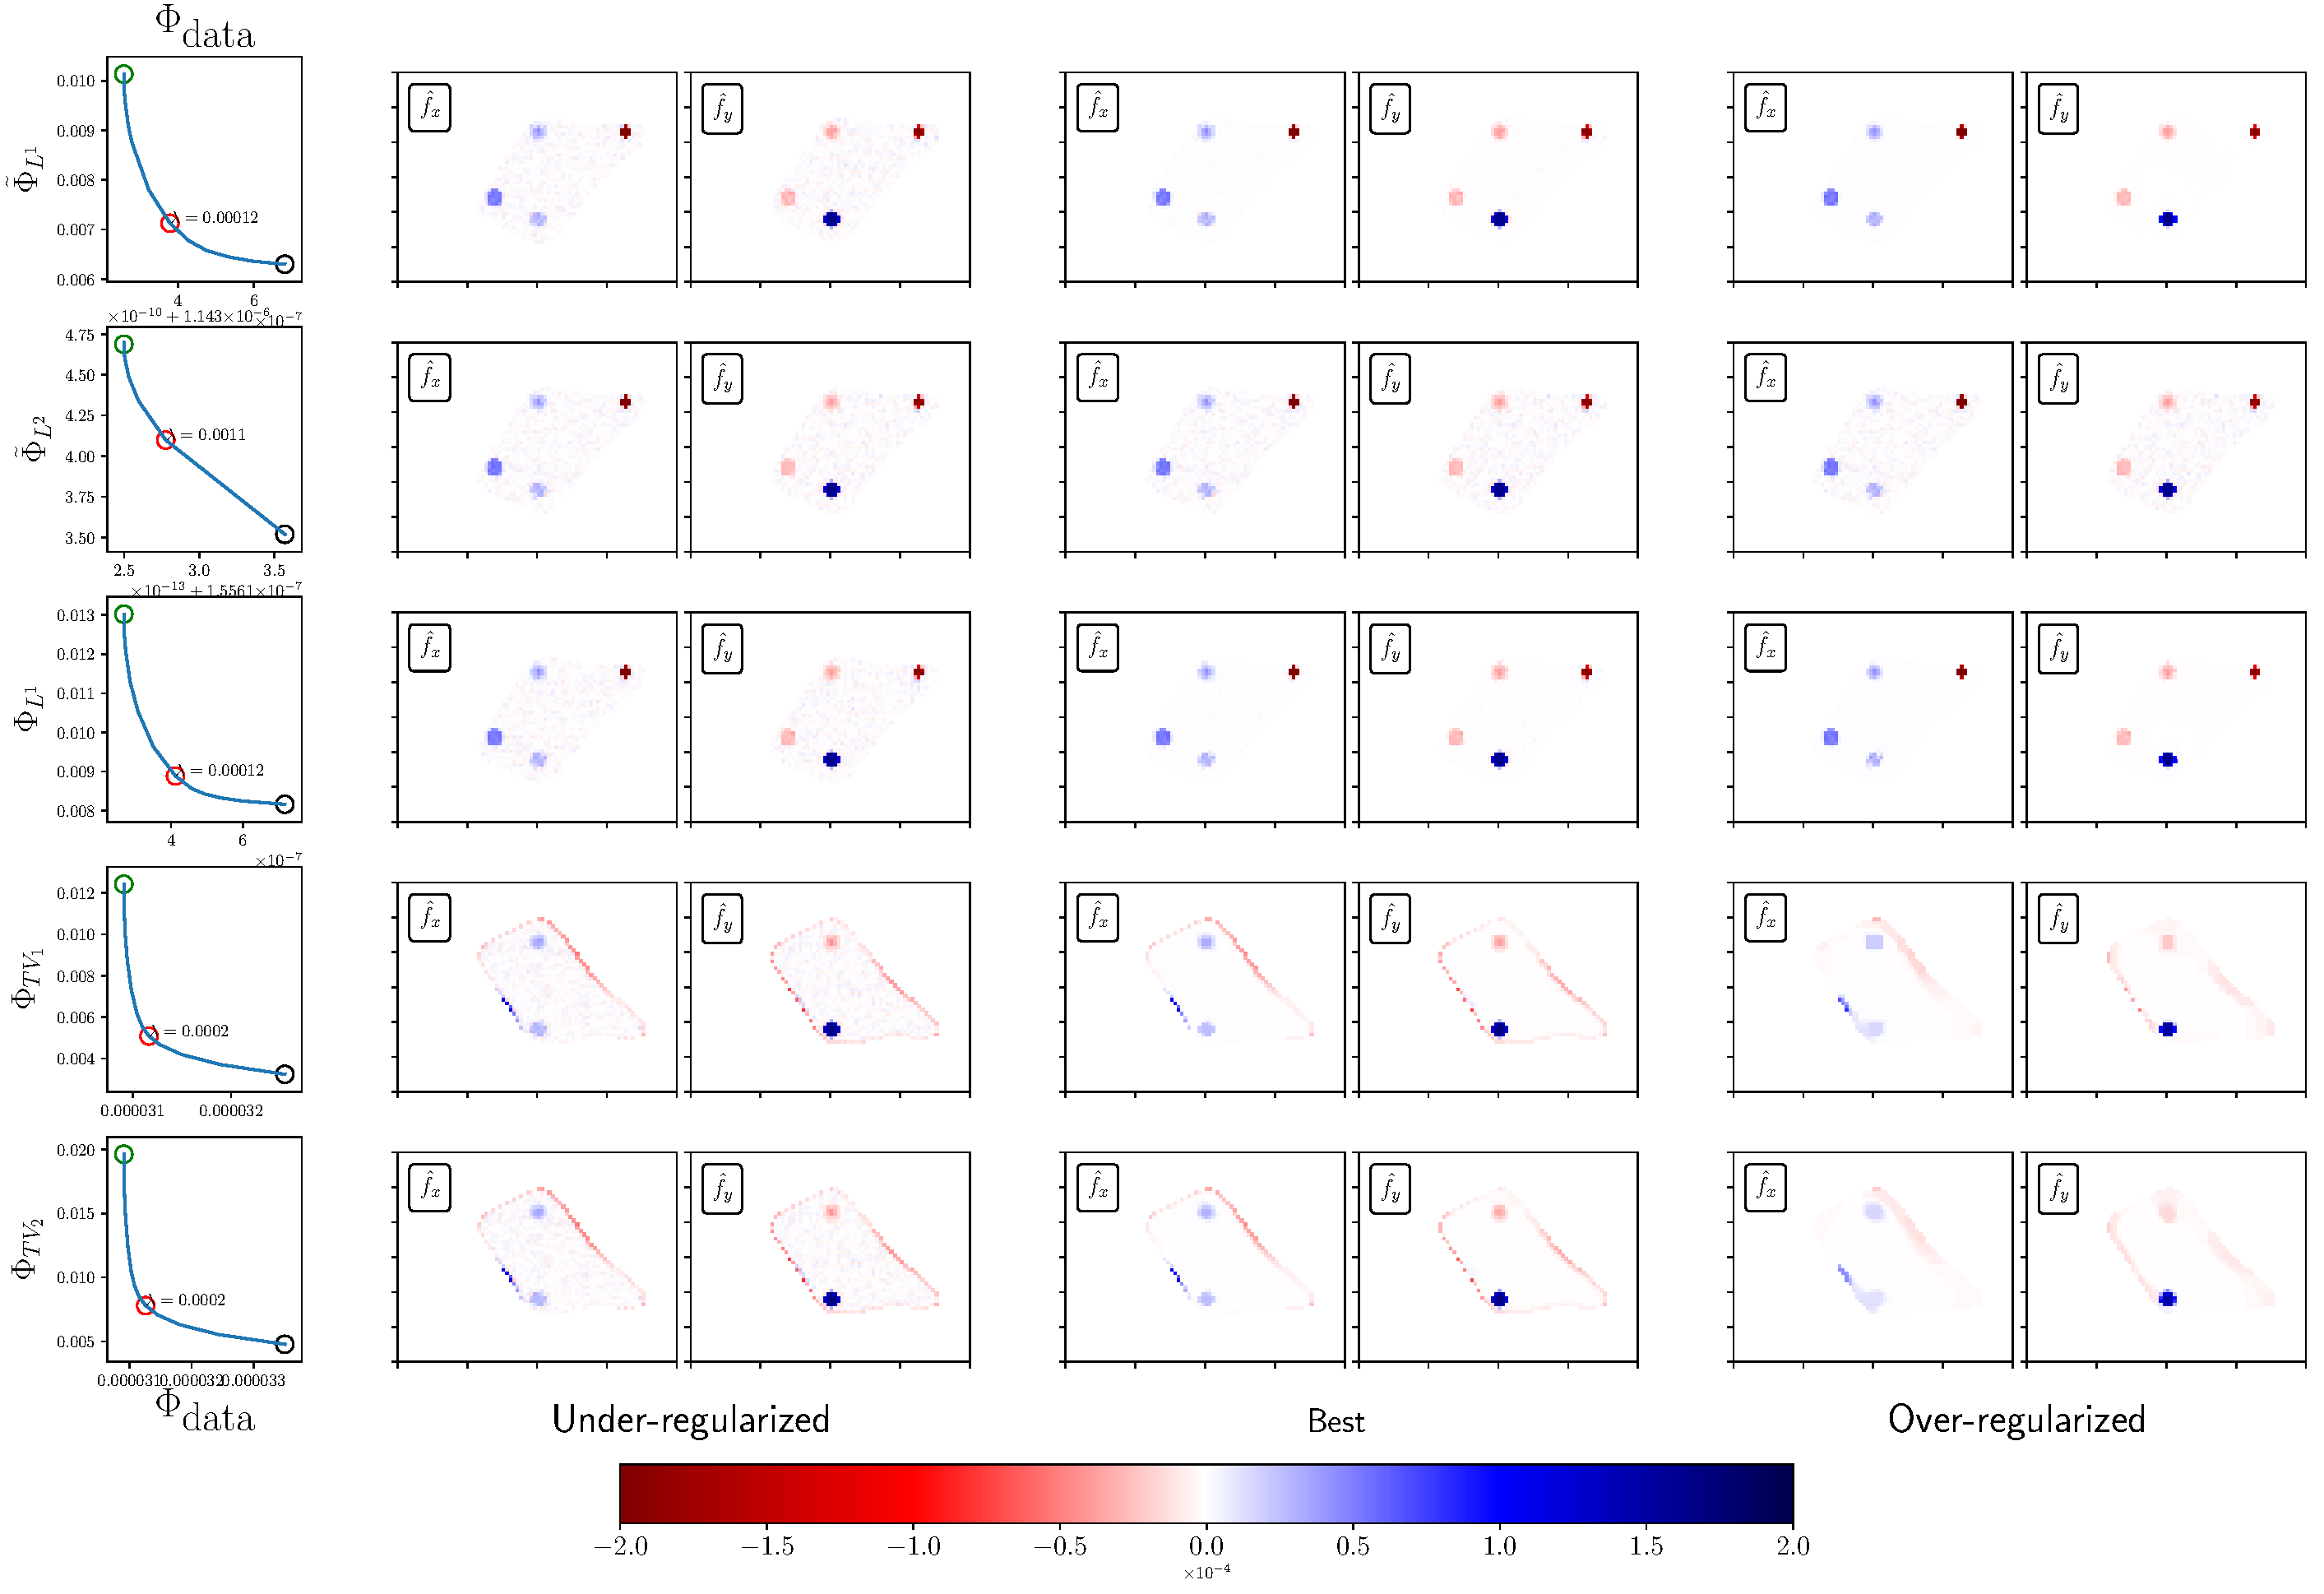
\includegraphics[width=\linewidth]{fig3}
\caption{\textbf{Omission of constraints} leads to solutions that do
  not naturally obey the constraints. Plotted are best reconstructions
  under the isotropic $L^1$ penalty and the difference between these
  reconstructions and the corresponding fully constrained
  reconstruction of Fig.~\ref{fig:fig2}. }
\label{fig:fig3}
\end{figure}

\begin{figure}
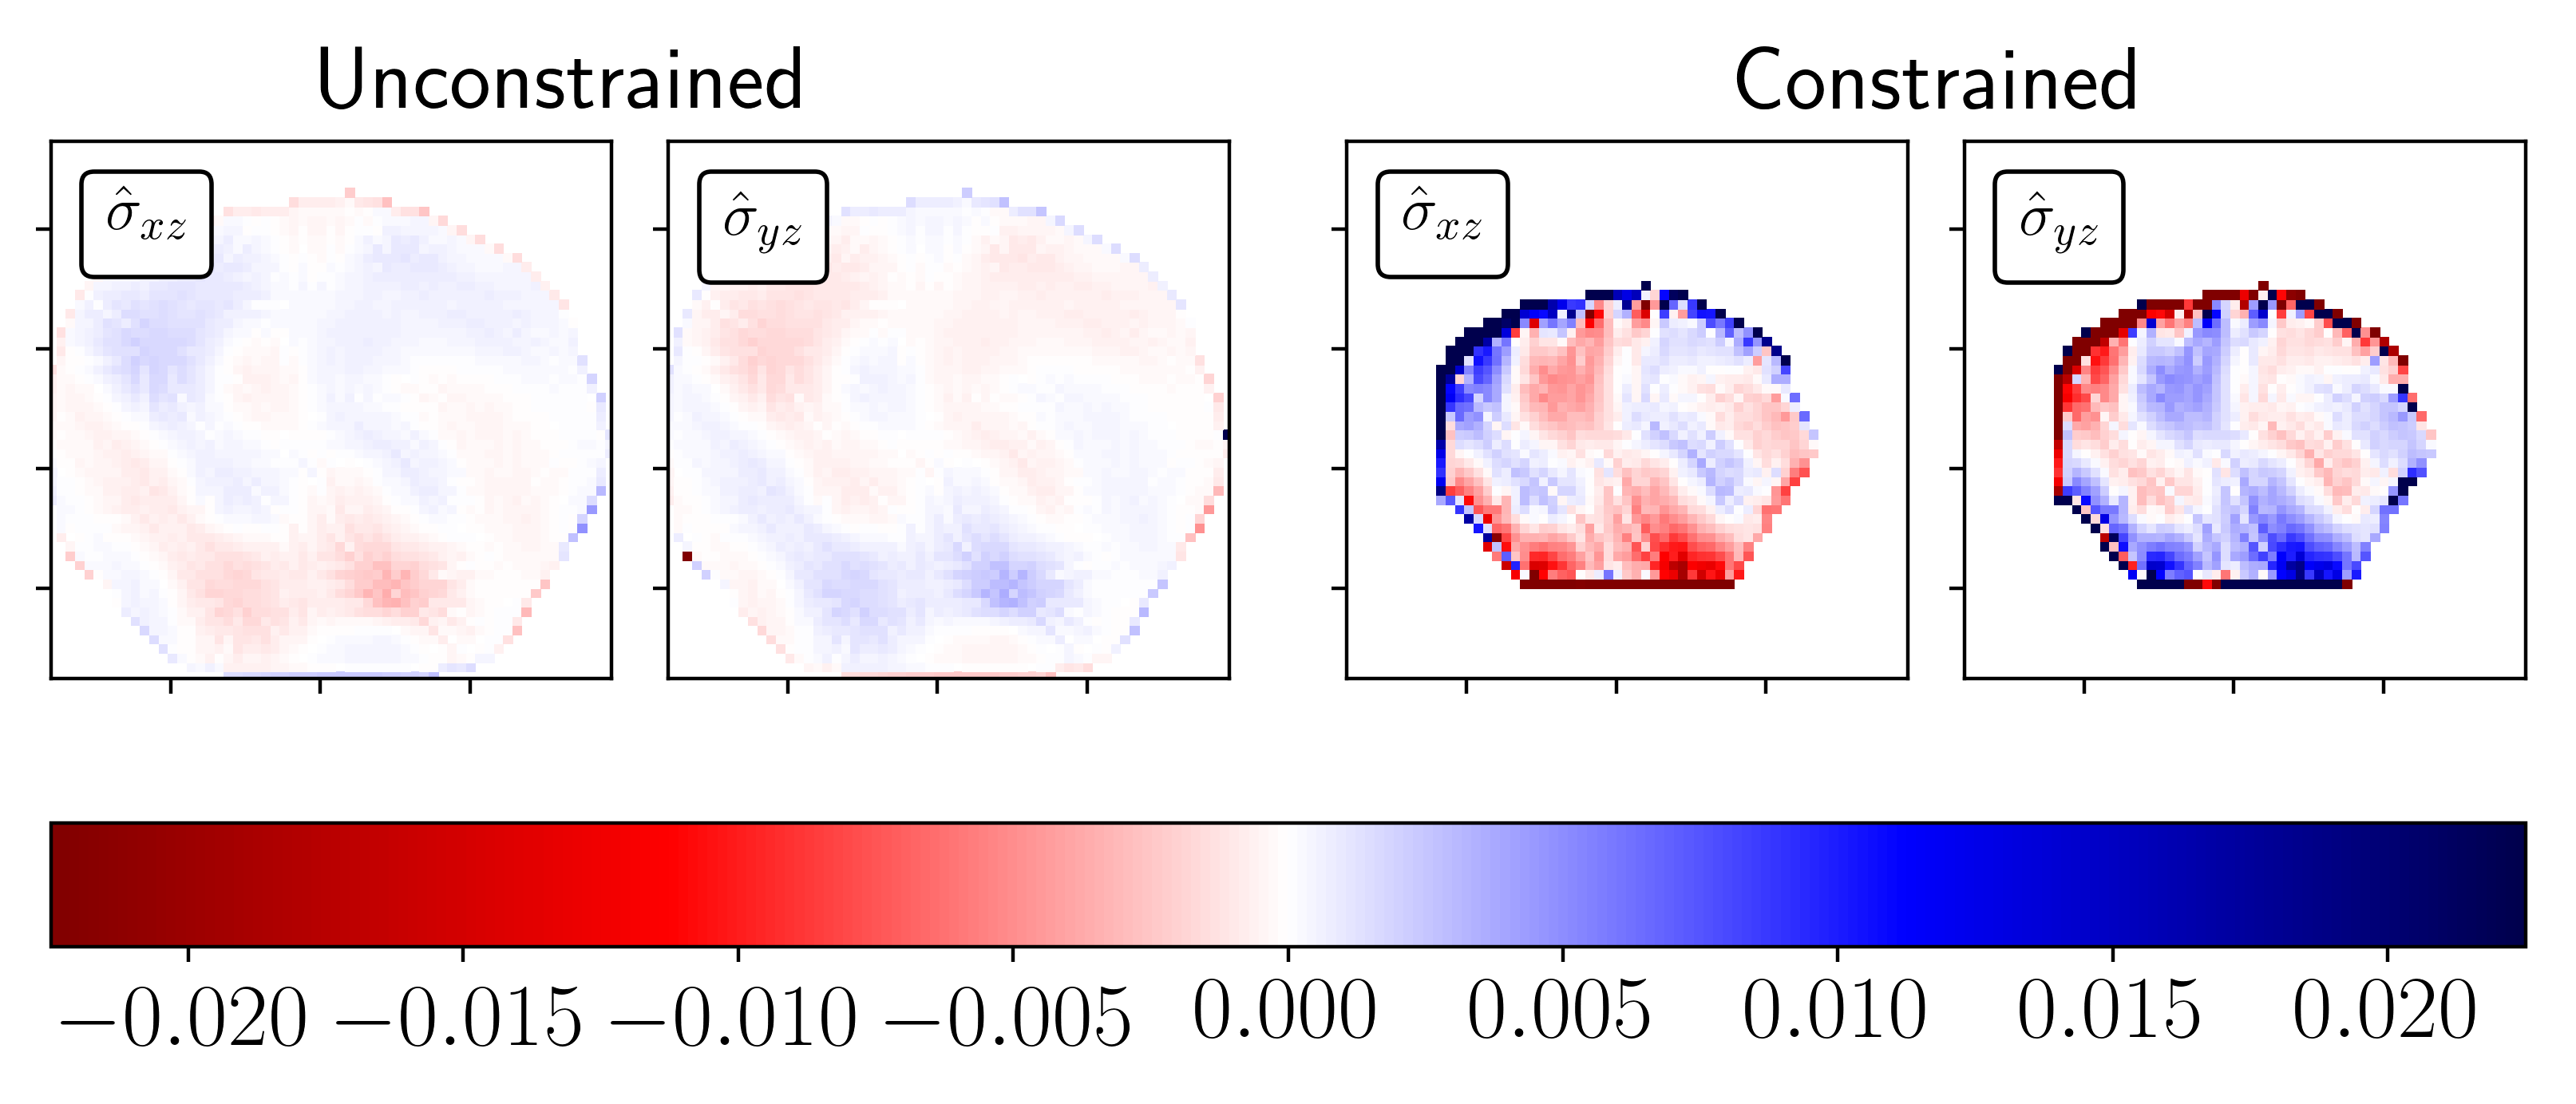
\includegraphics[width=\linewidth]{fig4}
\caption{\textbf{Boundary constraint weakening} leads to solutions
  where the support does not fall naturally within the cell
  boundary. In the unconstrained reconstruction, the support of the
  stress was allowed to extend an additional $10$ pixels outside of
  the cell boundary. The reconstruction did not naturally limit its
  support to the cell boundary.}
\label{fig:fig4}
\end{figure}


%%%%%%%%%%%%%%%%%%%%%%%%%%%%%%%%%%%%%%%%%%%%%%%%%%%%%%%%%%%%%%%%%%
\section{Discussion and Conclusions}
%%%%%%%%%%%%%%%%%%%%%%%%%%%%%%%%%%%%%%%%%%%%%%%%%%%%%%%%%%%%%%%%%%

We have presented a comprehensive method for solving the inverse
problem of surface stress reconstruction the incorporates physical
knowledge as constraints.  Under piecewise affine approximations of
the stress tensor, we provided an exact solution to the forward
problem as a system of linear equations. Using the multipole
expansion, we motivated the use of a cut-off in the solution of the
forward problem that greatly reduces the rank of the inverse problem
thereby decreasing both the computational complexity of the problem
and the memory requirements. The numerical stability of the problem
was also improved using regularization which obeys the geometric 
constraint that the problem should be rotationally invariant.

Our method exploits physical constraints that allows for superior
reconstruction of complex surface stress fields.  We also showed how
the known footprint boundary can imapct the reconstruction. In
general, footprints that extend beyond the extend of the support of
the stress field worsens the inversion, allowing for ``leakage'' of
stress beyond its actual support. Our method can naturally apply to
related systems such as scratch wound assays. 

\bibliography{refs}

\appendix

\section{Integrals }
In this section we provide closed-form expressions for the integrals represented by Eq.~\ref{eq:G_ave}.
Let $\Delta x_{nj}^+ = x_n - (x_j+\delta x/2),$ $\Delta x_{nj}^- = x_n - (x_j-\delta x/2),$ $\Delta y_{mk}^+ = y_m - (y_k+\delta y/2),$ and $\Delta y_{mk}^+ = y_m - (y_k-\delta y/2).$ Then,
we have the averaged Greens functions
\begin{align}
\langle G_{uv}\rangle^{nmjk} &=   f_{uv}( \Delta x_{nj}^+,\Delta y_{mk}^+) - f_{uv}( \Delta x_{nj}^+,\Delta y_{mk}^-)  \nonumber \\
&\qquad -f_{uv}(\Delta x_{nj}^-, \Delta y_{mk}^+) + f_{uv}(\Delta x_{nj}^- , \Delta y_{mk}^-)
\end{align}
where
\begin{align}\allowdisplaybreaks
f_{xx}(x,y) &= \frac{\nu+1}{\pi E}\Bigg[ x(1-\nu ) \log\left( \sqrt{x^2+y^2}+y\right) \nonumber\\
&\qquad+ y \log\left(\sqrt{x^2+y^2} +x\right)-y  \Bigg] \label{eq:fxx} \\
f_{yy}(x,y) &= \frac{\nu+1}{\pi E}\Bigg[ y(1-\nu ) \log\left( \sqrt{x^2+y^2}+x\right) \nonumber\\
&\qquad+ x \log\left(\sqrt{x^2+y^2} +y\right)-x  \Bigg] \label{eq:fyy} \\
f_{xy}(x,y) &= -\frac{\nu(\nu+1)}{\pi E}\sqrt{x^2+y^2}. \label{eq:fxy}
\end{align}
The first moments follow
\begin{align}
\lefteqn{\langle xG_{xx}(x,y) \rangle^{nmjk} =\Big[ f_{xx}( \Delta x_{nj}^+,\Delta y_{mk}^+)- f_{xx}( \Delta x_{nj}^+,\Delta y_{mk}^-)}\nonumber\\
 &\qquad\qquad\qquad   -f_{xx}(\Delta x_{nj}^-, \Delta y_{mk}^+)+ f_{xx}(\Delta x_{nj}^- , \Delta y_{mk}^-)\Big] x_n\nonumber\\
 &\quad\qquad\qquad   - \Big[ f^x_{xx}( \Delta x_{nj}^+ , \Delta y_{mk}^+)- f^x_{xx}( \Delta x_{nj}^+ , \Delta y_{mk}^-) \nonumber\\
 &\qquad\qquad\qquad-f^x_{xx}(\Delta x_{nj}^-, \Delta y_{mk}^+) + f^x_{xx}(\Delta x_{nj}^- , \Delta y_{mk}^-)\Big],
\end{align}
where
\begin{align}
f^x_{xx}(x,y) &= \frac{\nu+1}{2\pi E} \Big[ (\nu+1)y\sqrt{x^2 + y^2} \nonumber\\
&\qquad\qquad- (\nu-1) x^2\log\left(\sqrt{x^2 + y^2} +y  \right)  \Big],\label{eq:fxxx}
\end{align}
\begin{align}
\lefteqn{\langle yG_{xx}(x,y) \rangle^{nmjk} = \Big[f_{xx}( \Delta x_{nj}^+,\Delta y_{mk}^+) - f_{xx}( \Delta x_{nj}^+,\Delta y_{mk}^-) } \nonumber\\
&\qquad\qquad\qquad-f_{xx}(\Delta x_{nj}^-, \Delta y_{mk}^+) + f_{xx}(\Delta x_{nj}^- , \Delta y_{mk}^-)  \Big] y_m\nonumber\\
&\qquad\qquad - \Big[ f^y_{xx}(\Delta x_{nj}^+,\Delta y_{mk}^+) - f^y_{xx}(\Delta x_{nj}^+,\Delta y_{mk}^-)\nonumber\\
&\qquad\qquad - f^y_{xx}(\Delta x_{nj}^-,\Delta y_{mk}^+) + f^y_{xx}(\Delta x_{nj}^-,\Delta y_{mk}^-)  \Big],
\end{align}
where
\begin{align}
f^y_{xx}(x,y) &=\frac{\nu+1}{2\pi E} \Bigg[y^2\log\left(\sqrt{x^2+y^2}+x \right)  \nonumber\\
&\qquad- \sqrt{x^2+y^2}\left((2\nu-1)x + \frac{1}{2}\sqrt{x^2+y^2} \right)  \Bigg], \label{eq:fyxx}
\end{align}
and
\begin{align}
\lefteqn{\langle xG_{xy}(x,y) \rangle^{nmjk} = \Big[ f_{xy}(\Delta x_j^-, \Delta y_k^+) - f_{xy}(\Delta x_j^-,\Delta y_k^-) } \nonumber\\
&\qquad\qquad- f_{xy}(\Delta x_j^+,\Delta y_k^+) + f_{xy} (\Delta x_j^+,\Delta y_k^-) \Big]x_n\nonumber\\
&\qquad\qquad -   \Big[ f_{xy}^x(\Delta x_j^+,\Delta y_j^+) - f_{xy}^x(\Delta x_j^+,\Delta y_j^-) \nonumber\\
&\qquad\qquad- f_{xy}^x(\Delta x_j^-,\Delta y_j^+) + f_{xy}^x(\Delta x_j^-,\Delta y_j^-)\Big]
\end{align}
where
\begin{align}
f_{xy}^x(x,y) &=\frac{\nu(\nu+1)}{\pi E}\Big[ \frac{y^2}{2}\log\left(\sqrt{x^2+y^2} +x \right) \nonumber\\
&\qquad\qquad\qquad-\frac{1}{4}\sqrt{x^2+y^2}\left(\sqrt{x^2+y^2}+2x\right) \Big]. \label{eq:fxxy}
\end{align}
All of these expressions may be found through direct iterated evaluation of the integrals, noting that
as long as $n\neq m$ or $j\neq k$ the integrand (effectively the Green's function) is bounded, hence making
Fubini's theorem applicable given the compactly supported domains of integration.

In the 
special case where $n=m$ and $j=k$, these formulae also hold. This fact is found by decomposing the integration domain to
exclude the origin, for instance in the manner
\begin{equation}
\int_{ -\Delta y/2 }^{\Delta y/2 }\int_{- \Delta x/2 }^{\Delta x/2 } \d\r = \lim_{\varepsilon\to0} \left( \int_\varepsilon^{\Delta y/2}  +  \int_{-\Delta y/2}^\varepsilon   \right)\int_{\Delta x/2}^{\Delta x/2} \d\r.~\label{eq:splitdomain}
\end{equation}
Since the antiderivatives of Eqs~\ref{eq:fxx},~\ref{eq:fyy},~\ref{eq:fxy},~\ref{eq:fxxx},~\ref{eq:fyxx}, and~\ref{eq:fxxy} all have well-defined limits with only removable discontinuities at the origin,  integrals of the Green's functions defined through Eq.~\ref{eq:splitdomain} all converge about the origin and the equations above also hold in the case where $n=m$ and $j=k$.

\subsection{Proof of~Lemma \ref{lem:multipole}}

\begin{proof}
Note that $u_x$ and $u_y$ are symmetric in form. Hence, it will suffice to prove just one of these assertions. Eq.~\ref{eq:UMODEL1x} can be written as
\begin{align}
u_x(\r) &= \frac{1+\nu}{\pi E} \int \frac{\dd \r}{|\r-\r'|} \Bigg\{ \left[ \frac{\nu(x - x')^2}{|\r-\r'|^2} + 1-\nu \right]\sigma_{x}(\r')  \nonumber\\
&\quad+\nu\frac{(x-x')(y-y')}{|\r-\r'|^2} \sigma_y(\r')  \Bigg\} \nonumber\\
&= \frac{1+\nu}{\pi E}   \int \rho(\r,\r')    \frac{\dd \r'}{|\r-\r'|} \label{eq:rhoeq}
\end{align}
where $\rho(\r,\r')$ is $\mathcal{O}(1)$ as $\vert\r\vert\to\infty$. Without loss of generality, we assume that the coordinate system is centered at some point $\mathbf{0}\in\Omega$. The Euclidean distances can then be represented through the binomial expansion,
\begin{align}
\frac{1}{|\r-\r'|^p} &= \frac{1}{|\r|^p}\frac{1}{\left(1 - \frac{2\r\cdot\r' - |\r'|^2}{|\r|^2} \right)^p } \nonumber\\
&= \frac{1}{|\r|^p}\sum_{k=0}^\infty {{p+k-1}\choose{k}} 
{\left( \underbrace{ \frac{2\r\cdot\r' - |\r'|^2}{|\r|^2}}_{\mathcal{O}(|\r|^{-1})} \right)}^k,
\end{align} 
where the series converges due to the fact that $|\r| > |\r'|$, since $\r\not\in\Omega$, whereas $\r'\in\Omega$. Plugging this series into the last line of Eq.~\ref{eq:rhoeq}, one sees that it in order to show that the magnitude of $u_x(\r)$ is $\mathcal{O}(|\r|^{-2})$, it suffices to show that $\int \rho(\r,\r')\dd\r' \leq \mathcal{O}(|\r|^{-1})$.

Using the fact that $\int \bsigma(\r)\d\r = \mathbf{0}$, one finds that
%
\begin{align}
\lefteqn{\int \rho(\r,\r')\d\r'  =  \int (1-\nu)\sigma_x(\r')\d\r'}\nonumber\\
&\quad+\nu\int\left[ \frac{(x - x')^2}{|\r-\r'|^2} \sigma_{x}(\r') +  \frac{(x-x')(y-y')}{|\r-\r'|^2} \sigma_y(\r')  \right]\d\r' \nonumber\\
%&=\frac{\nu}{|\r|^2}\int\left[ \frac{(x - x')^2\sigma_{x}(\r')  + (x-x')(y-y')\sigma_y(\r') }{1- \frac{2\r\cdot\r' - |\r'|^2}{|\r|^2}} \right]\d\r' \nonumber\\
&= \frac{\nu}{|\r|^2}\int\Bigg[  (x - x')^2\sigma_{x}(\r')  + (x-x')(y-y')\sigma_y(\r')  \Bigg] \nonumber\\
&\qquad\qquad\qquad\times\sum_{k=0}^\infty \left[  \frac{2\r\cdot\r' - |\r'|^2}{|\r|^2} \right]^k \d\r'.
\end{align}
Expanding the leading order term of this expression, we see that
\begin{align*}
\lefteqn{\int\rho(\r,\r')\d\r } \nonumber\\
&= \frac{\nu}{|\r|^2}\int\Bigg[  (x - x')^2\sigma_{x}(\r')  + (x-x')(y-y')\sigma_y(\r')  \Bigg] \nonumber\\
&\qquad\times[1+\mathcal{O}(|\r|^{-1}) ]\d\r' \nonumber\\
&= \frac{\nu}{|\r|^2}  \Bigg[  -2x\int x'\sigma_x(\r')\d\r'  + \int x'^2\sigma_x(\r')\d\r'  \nonumber\\
&\qquad  - x\int y' \sigma_y(\r') \d\r'- y\int x'\sigma_y(\r')\d\r' \nonumber\\
&\qquad\qquad + \int x'y' \sigma_y(\r') \d\r'\Bigg][1+\mathcal{O}(|\r|^{-1}) ]\nonumber\\
&=\mathcal{O}(|\r|^{-1}).
\end{align*}
Hence, it is evident that this integral of $\mathcal{O}(|\r|^{-2})$, where to the leading order we have
\begin{align}
\lefteqn{u_x(\r) = \frac{1+\nu}{\pi E |\r|^2}\Bigg[ -2\frac{x}{|\r|}\int x'\sigma_x(\r')\d\r' - \frac{x}{|\r|}\int y' \sigma_y(\r') \d\r'  }\nonumber\\
&\qquad- \frac{y}{|\r|}\int x'\sigma_y(\r')\d\r' + 1-\nu \Bigg],
\end{align}
ignoring the fact that this expression also contains some information at lower orders.

% and $\cos\theta = \frac{(\r-\r_0,\r'-\r_0)} {|\r - \r_0| |\r'-\r_0|}$. Eq.~\ref{eq:multipole}  is obtained through binomial expansion of the Euclidean distance functions in the denominators of Eq.~\ref{eq:Gzz0} and Eq.~\ref{eq:Gxy0},
%\begin{align*}
%\lefteqn{|\r - \r'|^s = |\r-\r_0 - (\r'-\r_0) |^s }\\
%&\quad= \left[ |\r-\r_0|^2 -2 (\r-\r_0)(\r'-\r_0) + |\r'-\r_0|^2  \right]^{s/2}.
%\end{align*}
%In particular, since all the Green's functions scale with distance as $|\r-\r'|^{-1}$, we have the following approximation through the binomial expansion
%\begin{align}
%\lefteqn{\frac{1}{|\r-\r'|} =} \nonumber\\
%&  \frac{1}{|\r-\r_0|}\sum_{n=0}^\infty {n-\frac{1}{2} \choose n} \left[  \frac{2 (\r-\r_0)(\r'-\r_0) - |\r'-\r_0|^2 }{|\r-\r_0|} \right]^n \nonumber\\
%&=\frac{1}{|\r-\r_0|}\Bigg\{ 1 +    \frac{2 (\r-\r_0)(\r'-\r_0) - |\r'-\r_0|^2 }{2|\r-\r_0|}    \nonumber\\
%&\qquad+ \mathcal{O}(|\r-\r_0|^{-2})\Bigg\}.
%\end{align}
%Invoking the net force-free constraint, the first few terms of the expansion of Eq.~\ref{eq:multipole} are
%\begin{align}
%U_0 = 0
%\end{align}
\end{proof}
      
\subsection{Proof of~Lemma \ref{lem:affine_error}}

Let $\tilde{\bsigma}$ be the piecewise affine approximation of the stress field $\bsigma$, and $\r\in\Omega_{jk}$. Then,
by the Taylor remainder theorem, one sees that
$$
\sigma_{x}(\r) - \tilde{\sigma}_x(\r) = \frac{1}{2}(\r-\r_{jk})^\intercal\d^2\sigma_{x}(\mathbf{c}_{jk})(\r-\r_{jk})
$$
and
$$
\sigma_{y}(\r) - \tilde{\sigma}_x(\r) = \frac{1}{2}(\r-\r_{jk})^\intercal\d^2\sigma_{x}(\mathbf{a}_{jk})(\r-\r_{jk})
$$
where $\mathbf{c}_{jk},\mathbf{a}_{jk}\in\Omega_{jk}$ and $\r_{jk}\in\Omega_{jk}$ is the point about which interpolation is performed.
Hence,
\begin{align}
\lefteqn{u_x(\r) - \tilde{u}_x(\r)  = \sum_{j,k}\int_{\Omega_{jk}} G_{xx} (\r,\r')(\sigma_{x}(\r') - \tilde{\sigma}_x(\r')) \d\r } \nonumber\\
&\qquad+\sum_{j,k}\int_{\Omega_{jk}} G_{xy} (\r,\r')(\sigma_{y}(\r') - \tilde{\sigma}_y(\r')) \d\r \nonumber\\
&= \sum_{j,k} \frac{\d_{xx}^2\sigma_x(\mathbf{c}_{jk})}{2}\int_{\Omega_{jk}} G_{xx}(x-x',y-y')  (x'-x_j)^2 \d\r \nonumber\\
&  + \sum_{j,k} {\d_{xy}^2\sigma_x(\mathbf{c}_{jk})}\int_{\Omega_{jk}} G_{xx}(x-x',y-y')  (x'-x_j)(y'-y_k)\d\r \nonumber\\
&\quad + \sum_{j,k} \frac{\d_{yy}^2\sigma_x(\mathbf{c}_{jk})}{2}\int_{\Omega_{jk}} G_{xx}(x-x',y-y')  (y'-y_k)^2\d\r \nonumber\\
&\quad + \sum_{j,k} \frac{\d_{xx}^2\sigma_y(\mathbf{a}_{jk})}{2}\int_{\Omega_{jk}} G_{xy}(x-x',y-y')  (x'-x_j)^2\d\r \nonumber\\
&  + \sum_{j,k} {\d_{xy}^2\sigma_y(\mathbf{a}_{jk})}\int_{\Omega_{jk}} G_{xy}(x-x',y-y')  (x'-x_j)(y'-y_k)\d\r \nonumber\\
&\quad + \sum_{j,k} \frac{\d_{yy}^2\sigma_y(\mathbf{a}_{jk})}{2}\int_{\Omega_{jk}} G_{xy}(x-x',y-y')  (y'-y_k)^2\d\r 
\end{align}

\subsection{Proof of~Theorem \ref{thm:main}}

Consider the data penalty term $\Phi_{\textrm{data}}$ of the optimization problem
\begin{align*}
\Phi_{\rm data}[\bs] &=\sum_{i=1}^{M}\vert \u^{\rm
  data}(\r_{i})- \u(\r_i)\vert^{2}  + \sum_{i=M+1}^{N}\vert \u^{\rm
  data}(\r_{i})- \u(\r_i)\vert^{2} 
\end{align*}
where the first $M$ data points are all within a maximal cut off distance of $R$ within the boundary of the cell and the remaining $N-M$ datapoints lie outside this distance.

%%%%%%%%%%%%%%%%%%%%%%%%%%%%%%%%%%%%%%%%%%%%%%%%%%%%%%%%%%%%%%%%%%%%%%%%
%%%%%%%%%%%%%%%%%%%%%%%%%%%%%%%%%%%%%%%%%%%%%%%%%%%%%%%%%%%%%%%%%%%%%%%%
\end{document}
%%%%%%%%%%%%%%%%%%%%%%%%%%%%%%%%%%%%%%%%%%%%%%%%%%%%%%%%%%%%%%%%%%%%%%%%
%%%%%%%%%%%%%%%%%%%%%%%%%%%%%%%%%%%%%%%%%%%%%%%%%%%%%%%%%%%%%%%%%%%%%%%%

